\headline{{\textbf{\Large\sffamily Bonsai Pots for Mame}}\\
          {\textbf{\large\sffamily By Alex Rudd}}}
\label{2025-04-pots}
\noindent
Alex Rudd (\href{https://www.europeanbonsaipottercollective.com}{European Bonsai Potter Collective}) delivered an engaging and informative talk on Mame bonsai pots, covering their unique qualities, history, influential potters, and their growing appeal in Europe.

Alex began by expressing his passion for bonsai pots, particularly Mame bonsai pots, which he finds the most enjoyable aspect of bonsai cultivation.
He noted that while pots for larger bonsai trees need to adhere to strict aesthetic principles, Mame pots offer greater creative freedom.

Two main reasons were given for this flexibility:

\begin{itemize}
    \item \textbf{Mame trees are difficult to keep alive} --- Their small size means they have minimal soil volume, requiring careful watering and maintenance.
    Because of this, using a slightly larger pot (relative to the tree size) is generally accepted.
    
    \item \textbf{They serve a different function in displays} --- Unlike larger bonsai pots, which emphasise the tree's characteristics, Mame pots contribute to the overall flow of a display, guiding the viewer's eye from tree to tree.
    This allows for more decorative and unconventional designs.
\end{itemize}

Mame bonsai pots, according to Alex, offer an exciting artistic opportunity, allowing for bolder colours, unusual shapes, and more intricate decorative elements than the often understated and refined aesthetic of larger bonsai pots.

\medskip

\topic{\large{Mame Bonsai Pots Rise in the 20th Century}}
\noindent
Alex then provided an overview of how Mame bonsai pots gained popularity, particularly in Japan from the 1950s to the 1970s.

\medskip

\topic{Key Figures in Mame Bonsai Pottery}
\noindent
Two major enthusiasts from this era were:

\begin{itemize}
    \item \textbf{Count Matsudaira}
    \item \textbf{Zou Nakamura (or Zoakamura, depending on transcription errors)}
\end{itemize}

Both were avid collectors, each owning over 2,000 Mame trees.
Zou Nakamura was not just a collector but also a pot historian and maker, significantly influencing the appreciation of Mame pots.

During a small bonsai show in Kiryu in the 1960s, Nakamura encountered a young potter, \textbf{Fujioka Yoshimura} (or something similar).
Impressed by his work, Nakamura bought everything he had.
Word spread rapidly, and overnight, Fujioka became one of Japan's most celebrated bonsai potters.

\medskip

\topic{Innovative Pottery Techniques}
\noindent
One of Fujioka's standout styles was the \textbf{``Five\--Colour Glaze'} technique, which required multiple firings in the kiln to achieve vibrant, layered hues.
This showcased the increasing artistic ambition within Mame bonsai pottery.

\medskip

\topic{\large{The Yokohama Guild and the Debate Over Mame Pot Styles}}
\noindent
By the 1970s, there was a divide in the bonsai community regarding the artistic direction of Mame bonsai pots.
Traditionalists argued that highly decorative pots distracted from the trees, while a new wave of potters embraced intricate carvings, paintings, and vibrant glazes.

Three potters formed \textbf{The Yokohama Guild} in 1974, meeting in the home of a potter named \textbf{Chowri (possibly Chōri or a similar name)}.
Their club focused on Mame bonsai and, significantly, Mame bonsai pots.
One of the founding members, \textbf{Okada Tetsuji (or a similar name)}, became well known for his detailed yet subtly elegant pot designs.

Okada's student, \textbf{Hashimoto Bunka (potentially ``Hashi Bunka'')}, continued this tradition, incorporating \textbf{repeating motifs}, such as a famous pot featuring a gradually shrinking line of monks—a humorous yet sophisticated design.

\medskip

\topic{\large{Key Potters and Their Contributions}}
% \noindent
% \medskip
\topic{Imeoka Masanori (or ``Imeokka Masin'')}
\noindent
\begin{itemize}
    \item Specialised in recreating traditional glazes with extreme accuracy.

    \item His \textbf{``Crawling Glaze''} (known in Japan as \textbf{Kiraku\--yu}) shrinks in the kiln, creating distinctive patterns.
    
    \item Also known for \textbf{Celadon (Seiji) glazes}, which give pots a translucent, jade\--like quality.
\end{itemize}

\medskip

\topic{Eno Shakuro}
\noindent
\begin{itemize}
    \item Part of a \textbf{three\--generation pottery lineage} dating back centuries.
    
    \item Produced highly refined \textbf{porcelain painted pots}, often with imperial \textbf{blue and yellow} colour schemes.
    
    \item His work was influenced by Chinese bonsai pot aesthetics, with long, thin\--walled designs.
\end{itemize}

\medskip

\topic{Ichiyuu (or ``Ichibaj''?) and His ``Kuriyuki'' Technique}
\noindent
\begin{itemize}
    \item Created pots by carving them from a solid block of clay, a process called \textbf{Kuriyuki}.
    
    \item This technique results in thin yet perfectly even pot walls, requiring exceptional skill.
\end{itemize}

\medskip

\topic{\large{The Increasing Rarity and Investment Value of Mame Bonsai Pots}}
\noindent
Alex highlighted that many of the pioneering Mame potters passed away in the late 20th century, making their work highly sought after.
Some specific cases he mentioned:

\begin{itemize}
    \item \textbf{Solidai Suki (possibly ``Sorida Suki'')} --- A highly revered potter, who passed away in 1985.
    Alex has been collecting his pots for over 10 years and has witnessed a surge in their value.

    \item One pot Alex purchased for \textbf{£600} was later valued at \textbf{£4,000}, although the market has since fluctuated, with prices currently around \textbf{£2,500}.
\end{itemize}

He also noted that American and European collectors have been increasingly driving up demand, with Chinese buyers in particular acquiring large quantities of rare pots.

\medskip

\begin{figure*}[!p]
\centering
\begin{minipage}[b]{.47\textwidth}
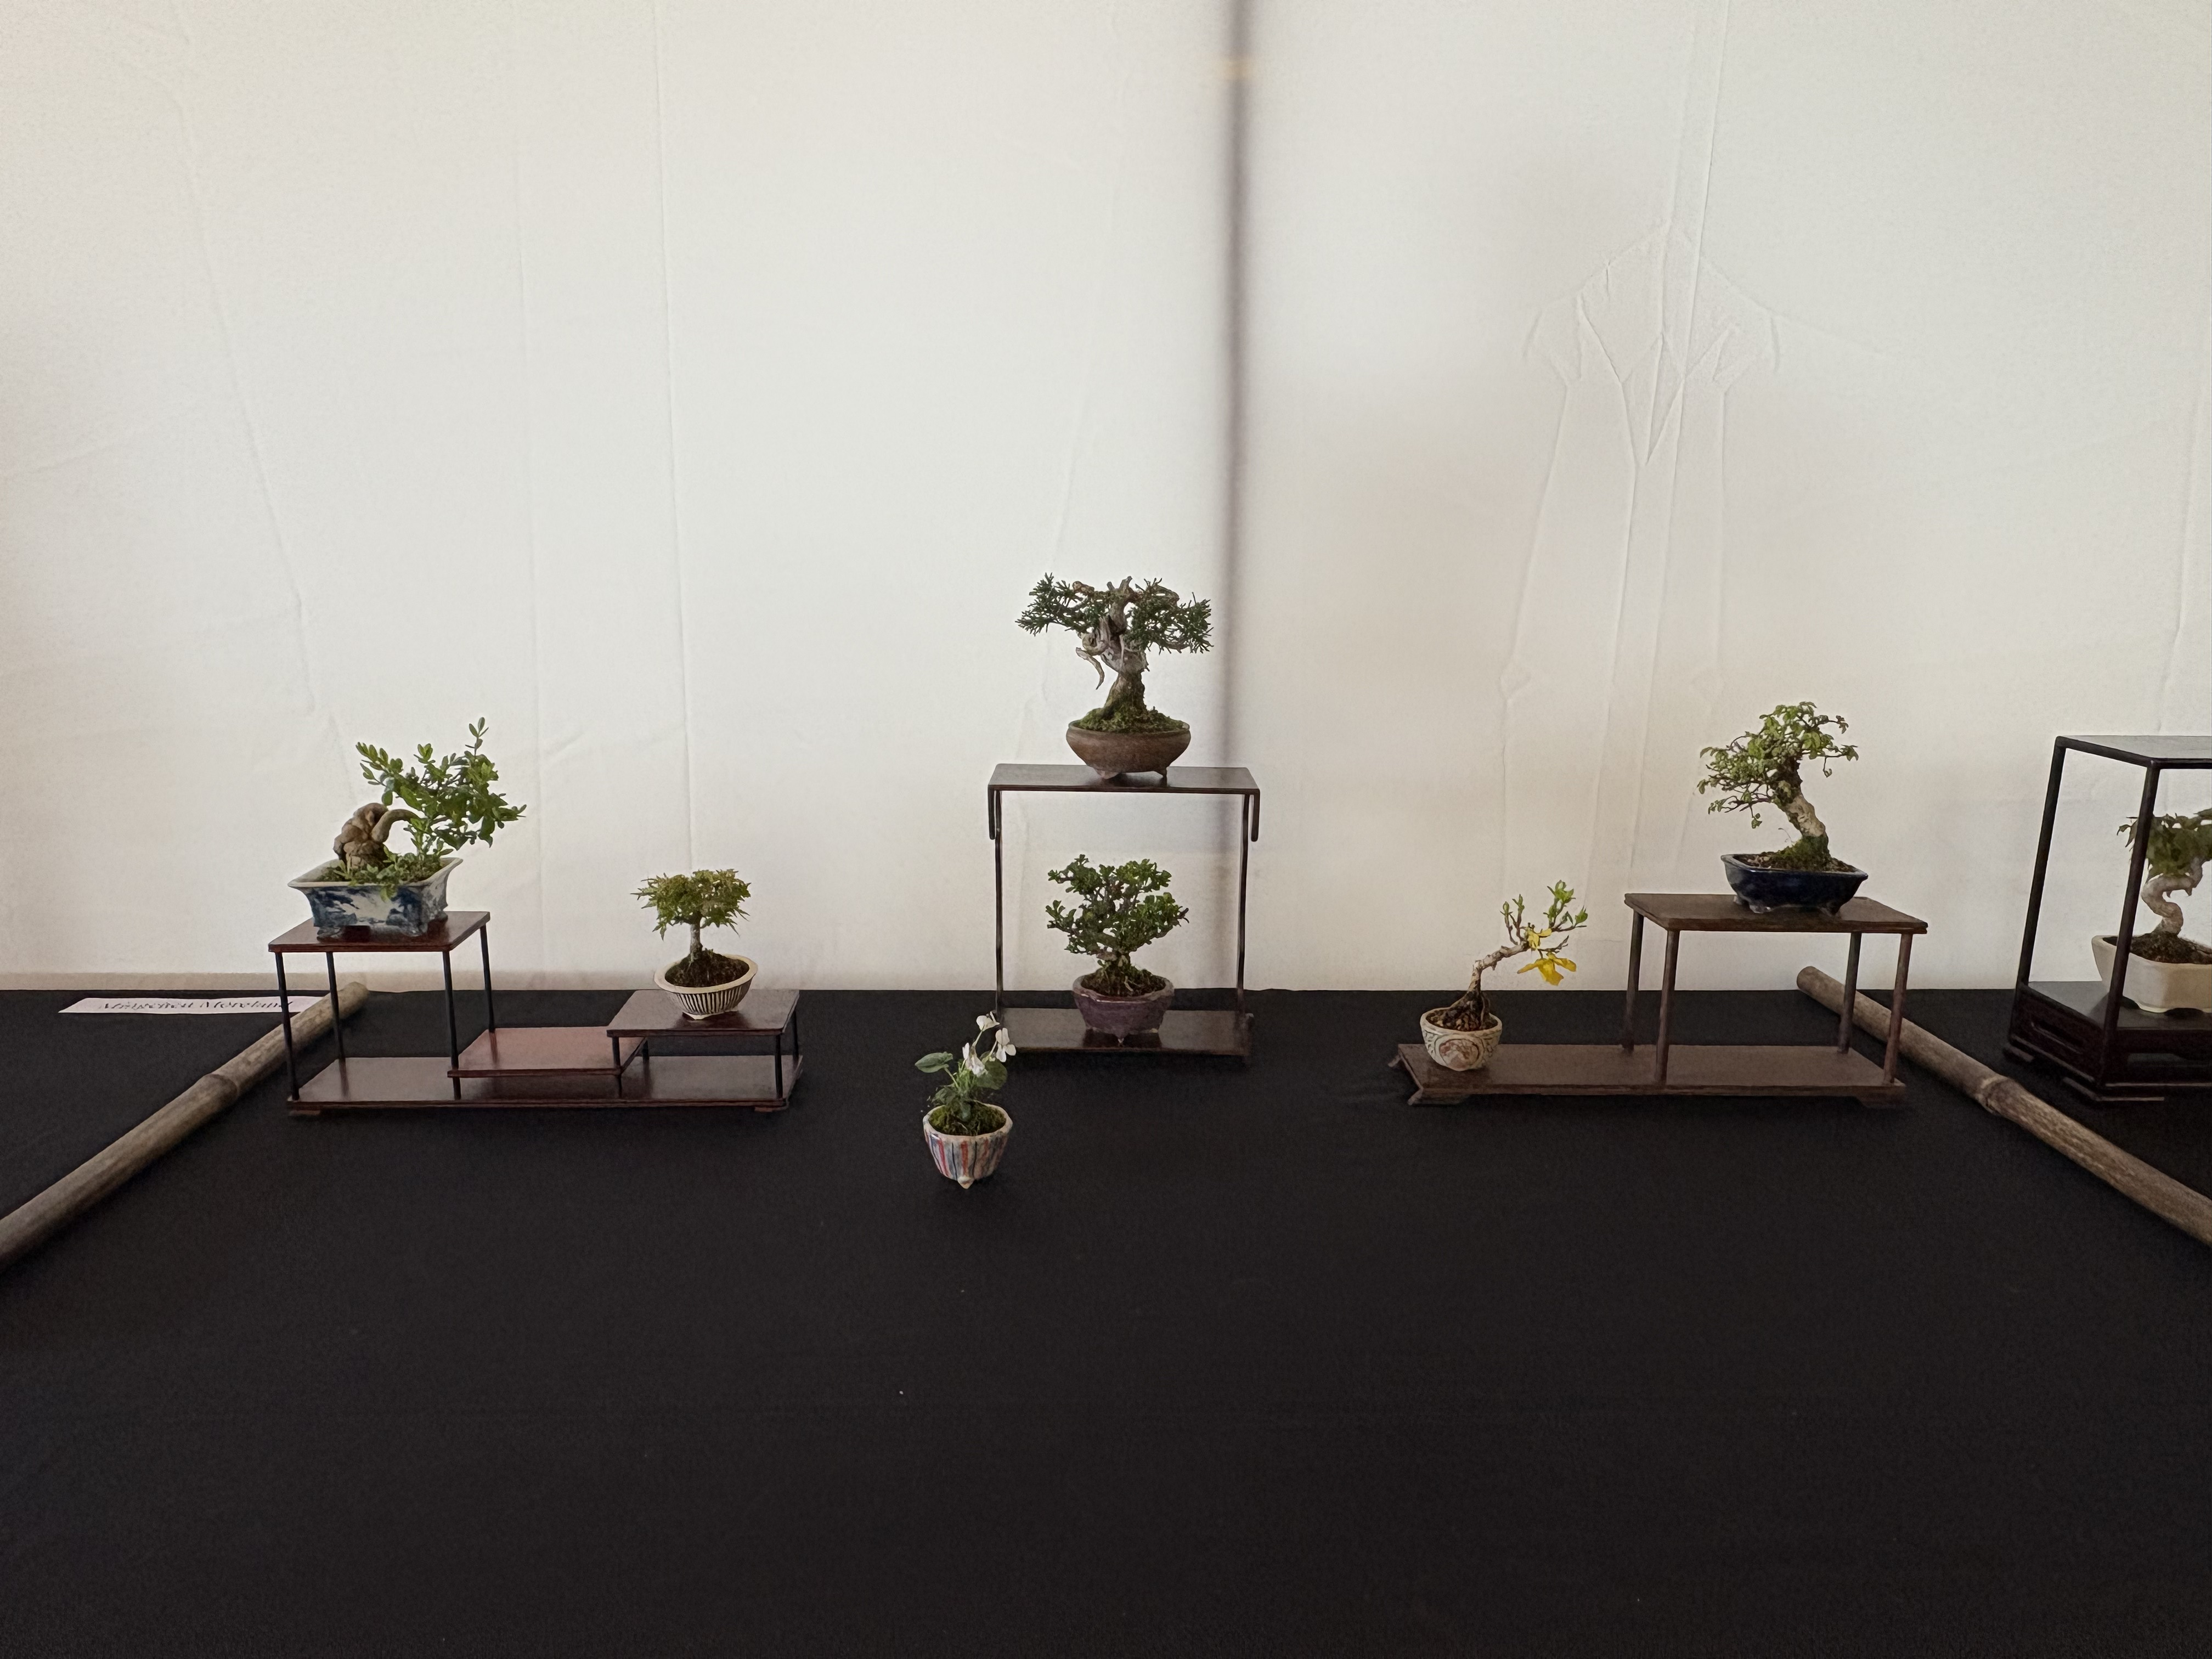
\includegraphics[width=1.0\textwidth]{2025_04/res/display_07}
% \centerline{\emph{David's Hawthorn.}}
\end{minipage}\qquad
\begin{minipage}[b]{.47\textwidth}
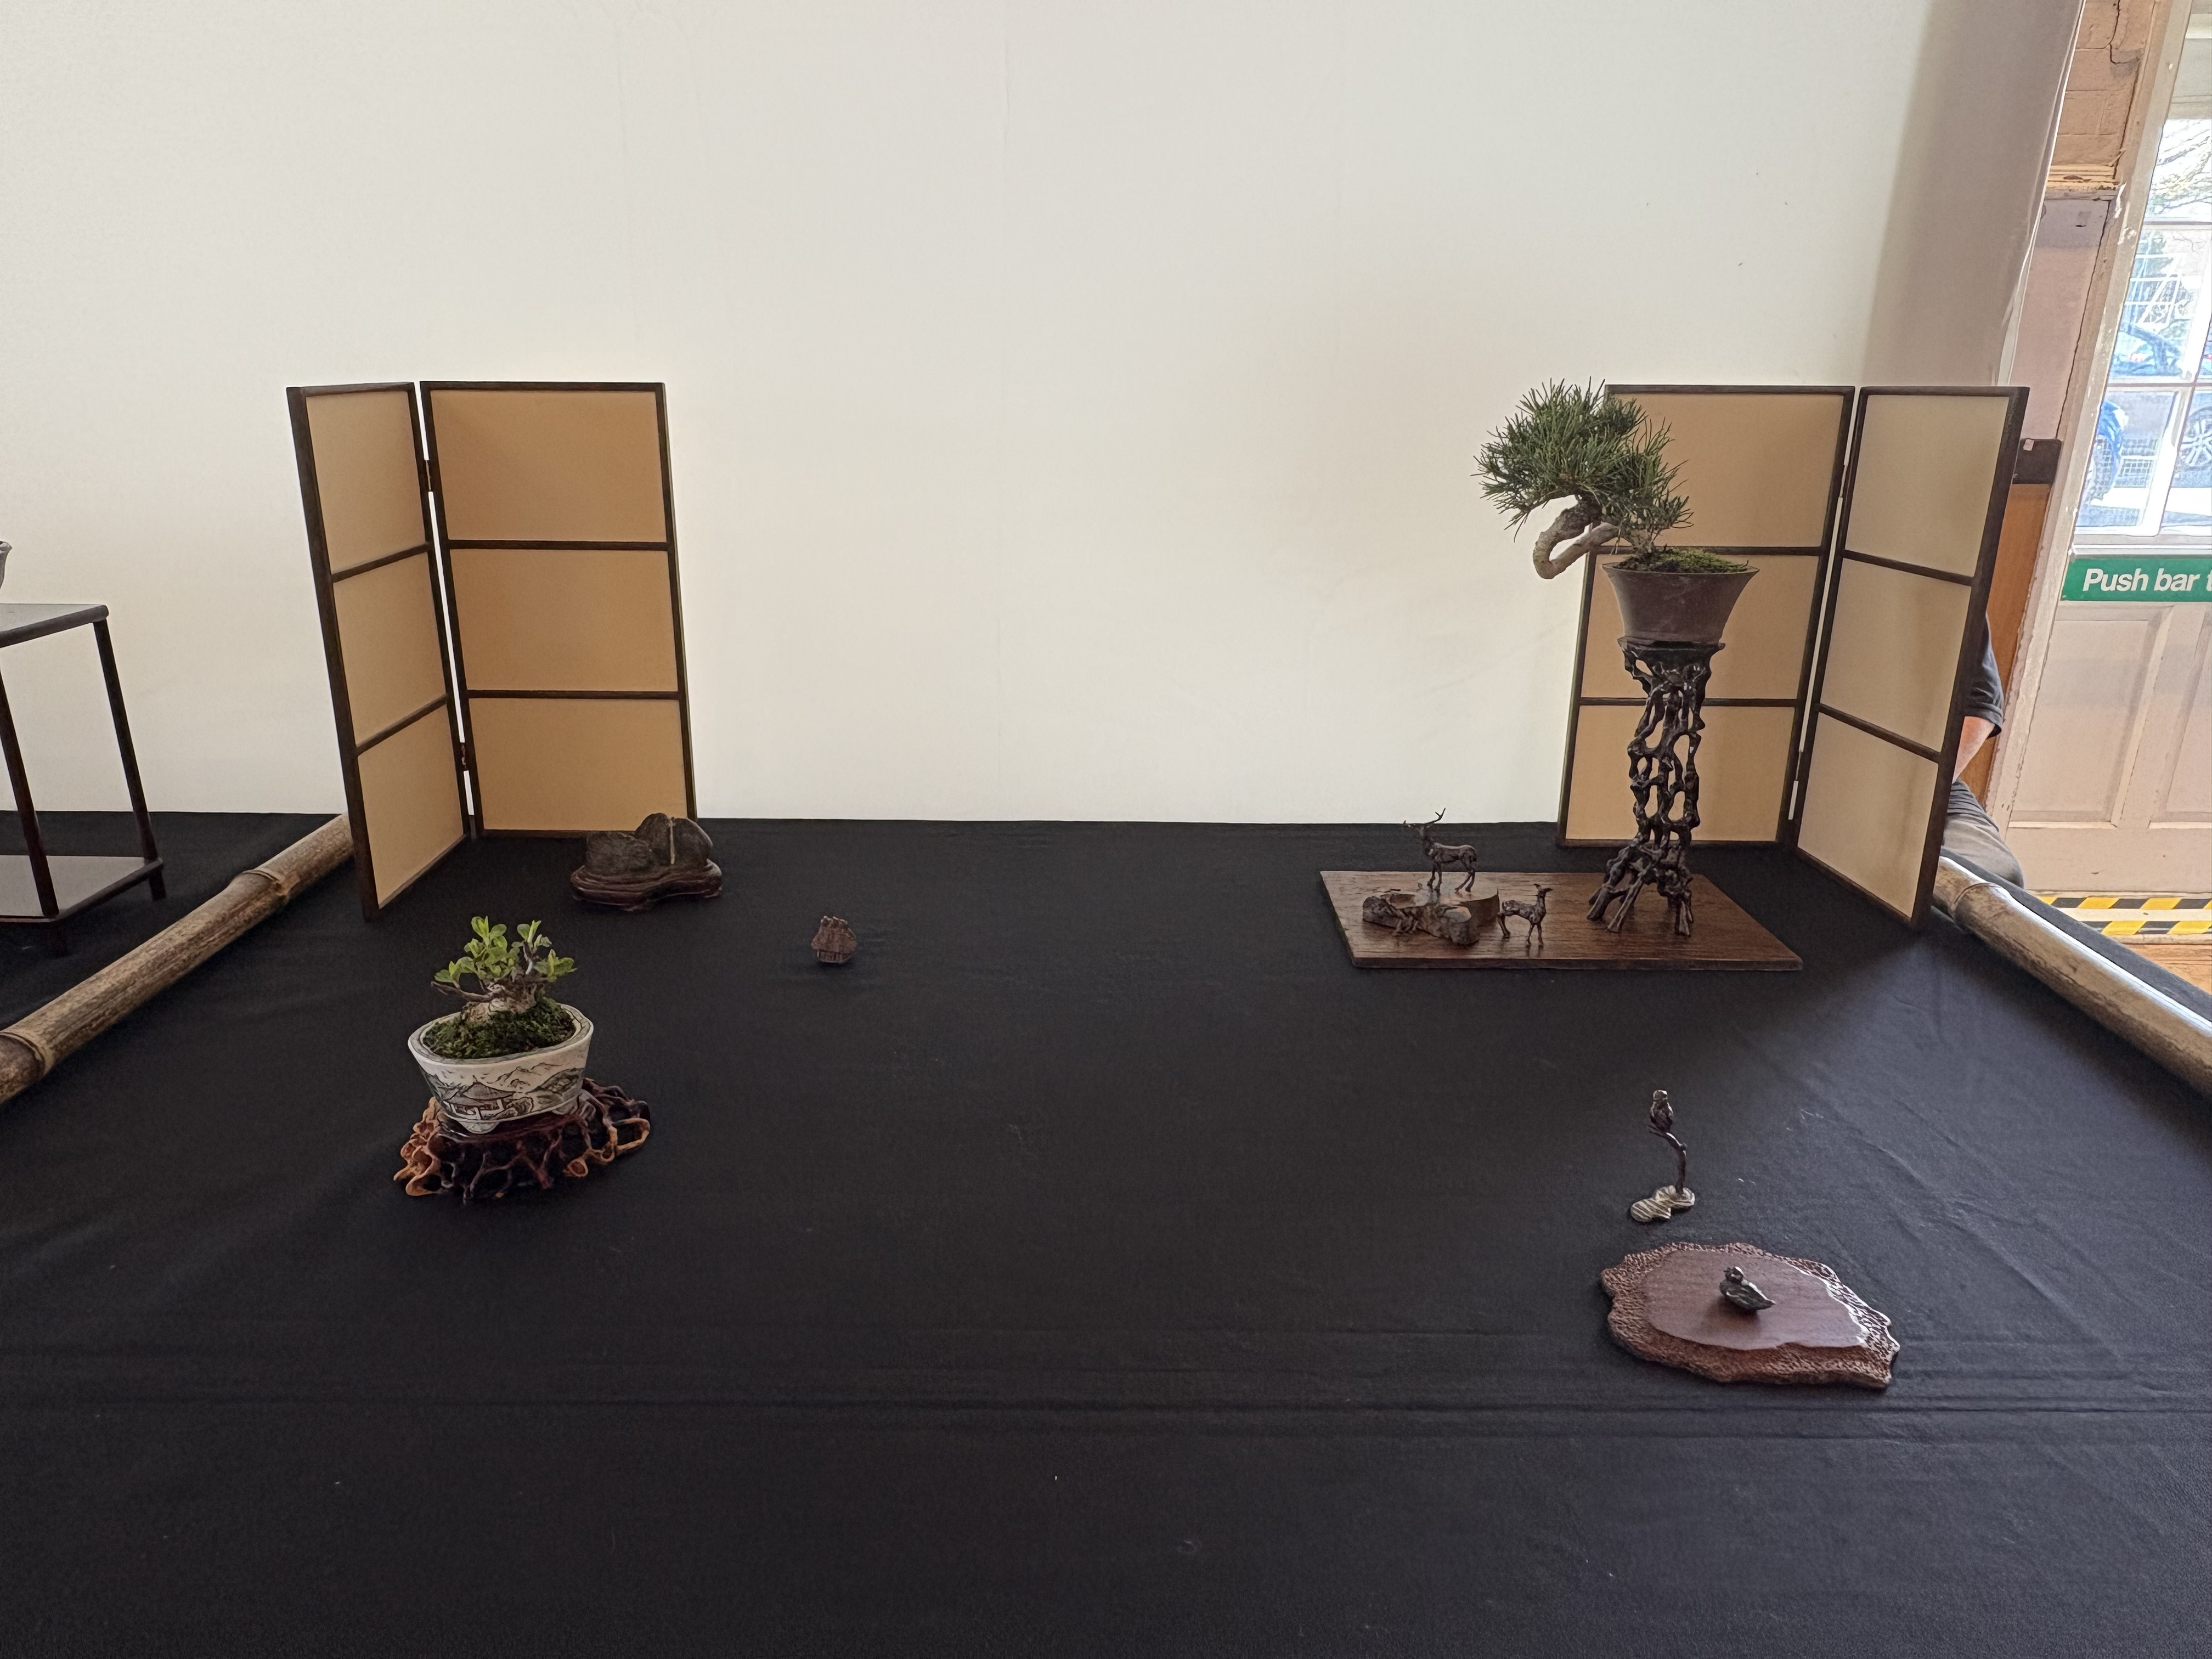
\includegraphics[width=1.0\textwidth]{2025_04/res/display_08}
% \centerline{\emph{Nick's Privet.}}
\end{minipage}
\medskip

\begin{minipage}[b]{.47\textwidth}
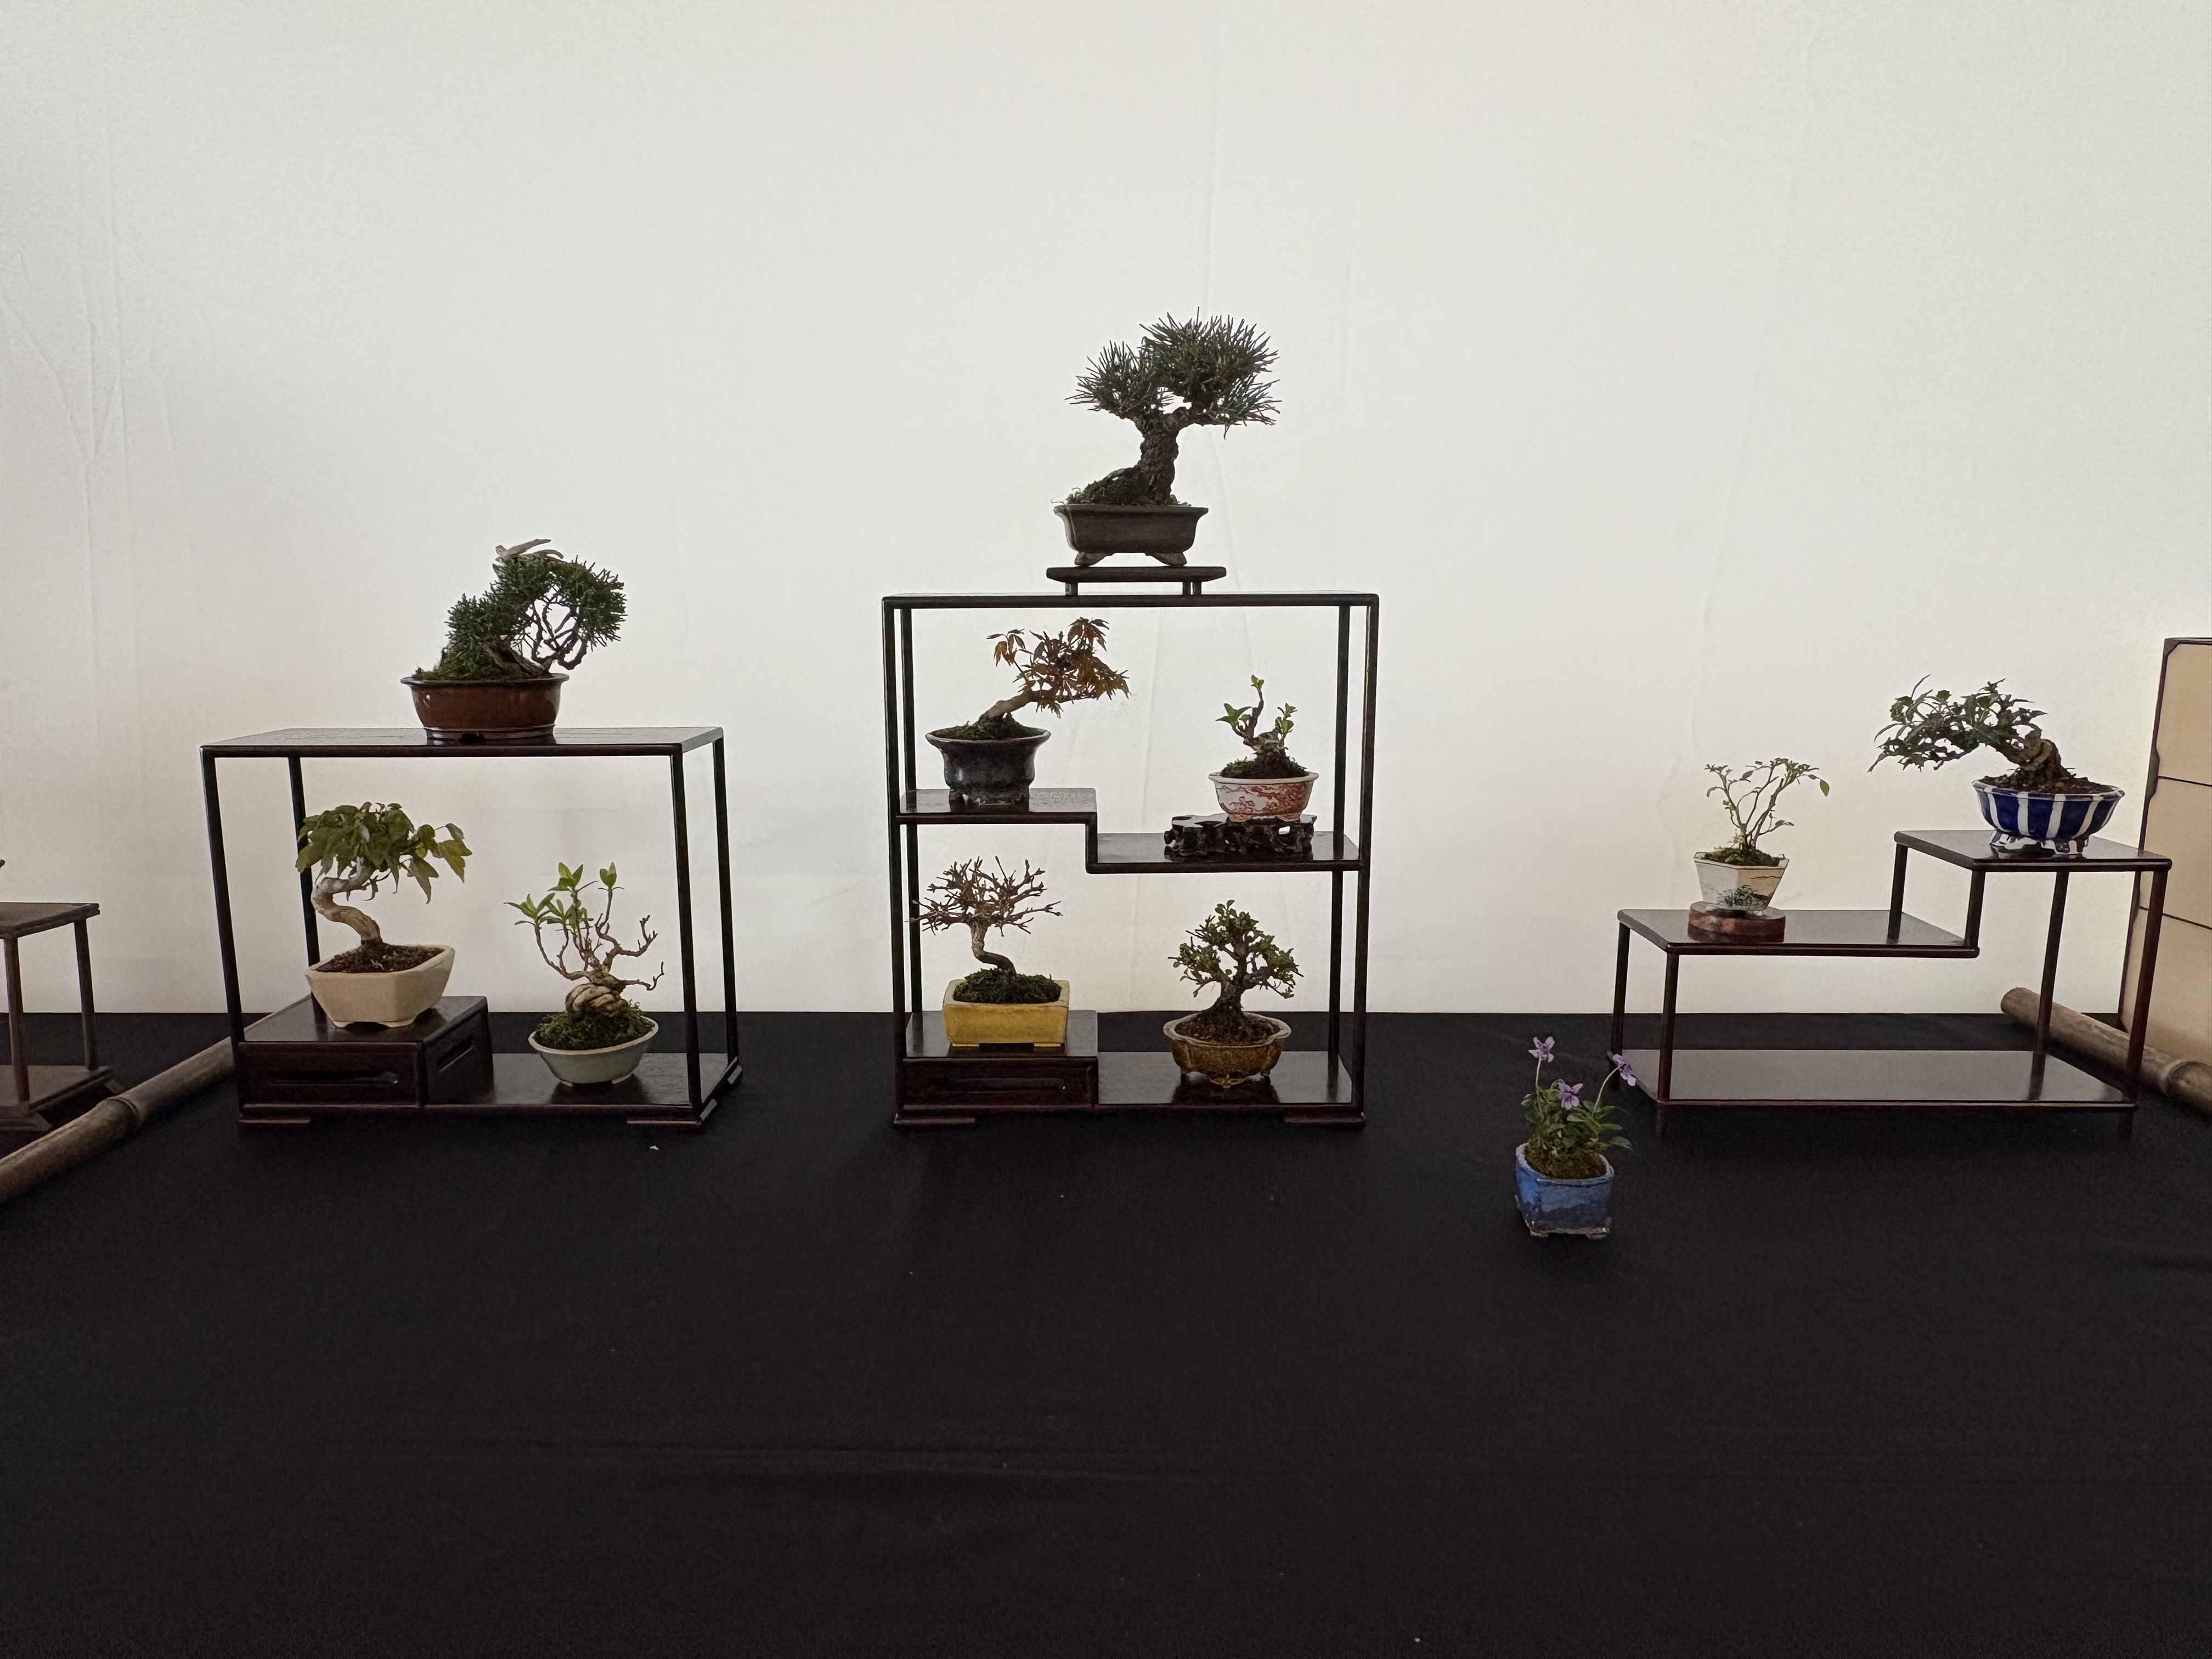
\includegraphics[width=1.0\textwidth]{2025_04/res/display_09}
% \centerline{\emph{Brendan's Yew.}}
\end{minipage}\qquad
\begin{minipage}[b]{.47\textwidth}
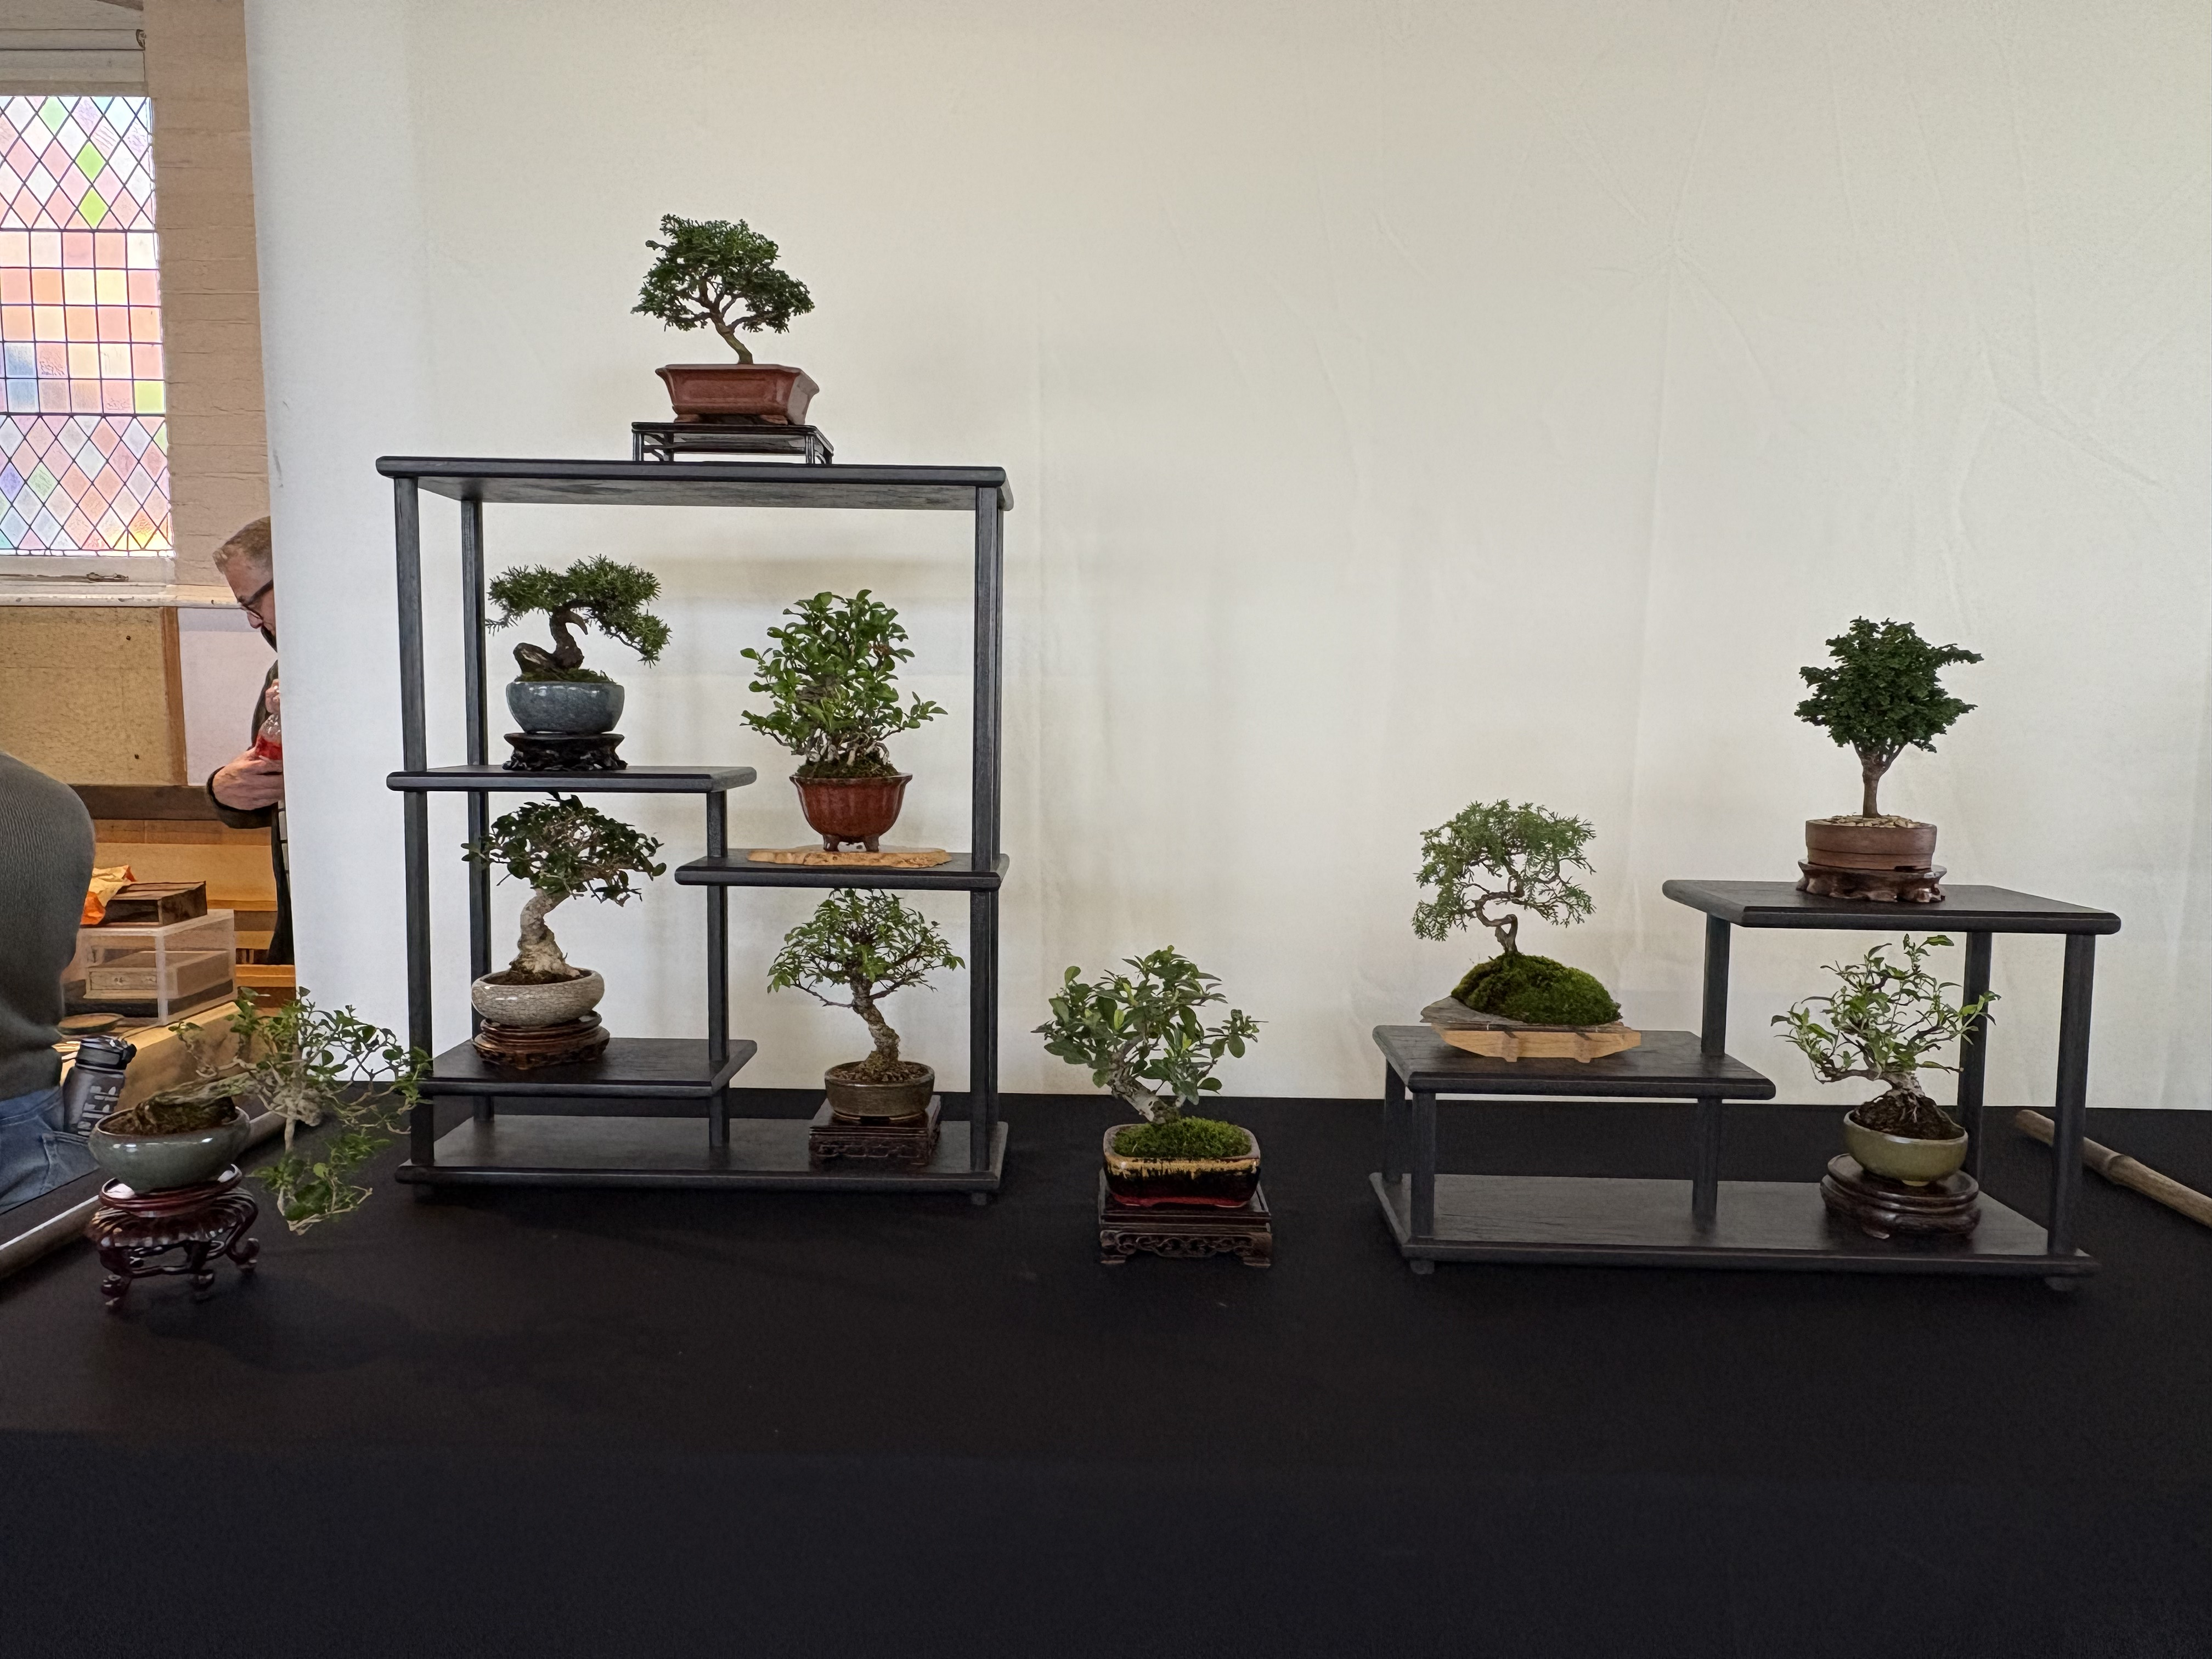
\includegraphics[width=1.0\textwidth]{2025_04/res/display_10}
% \centerline{\emph{Tony's Hawthorn.}}
\end{minipage}
\medskip

\begin{minipage}[b]{.47\textwidth}
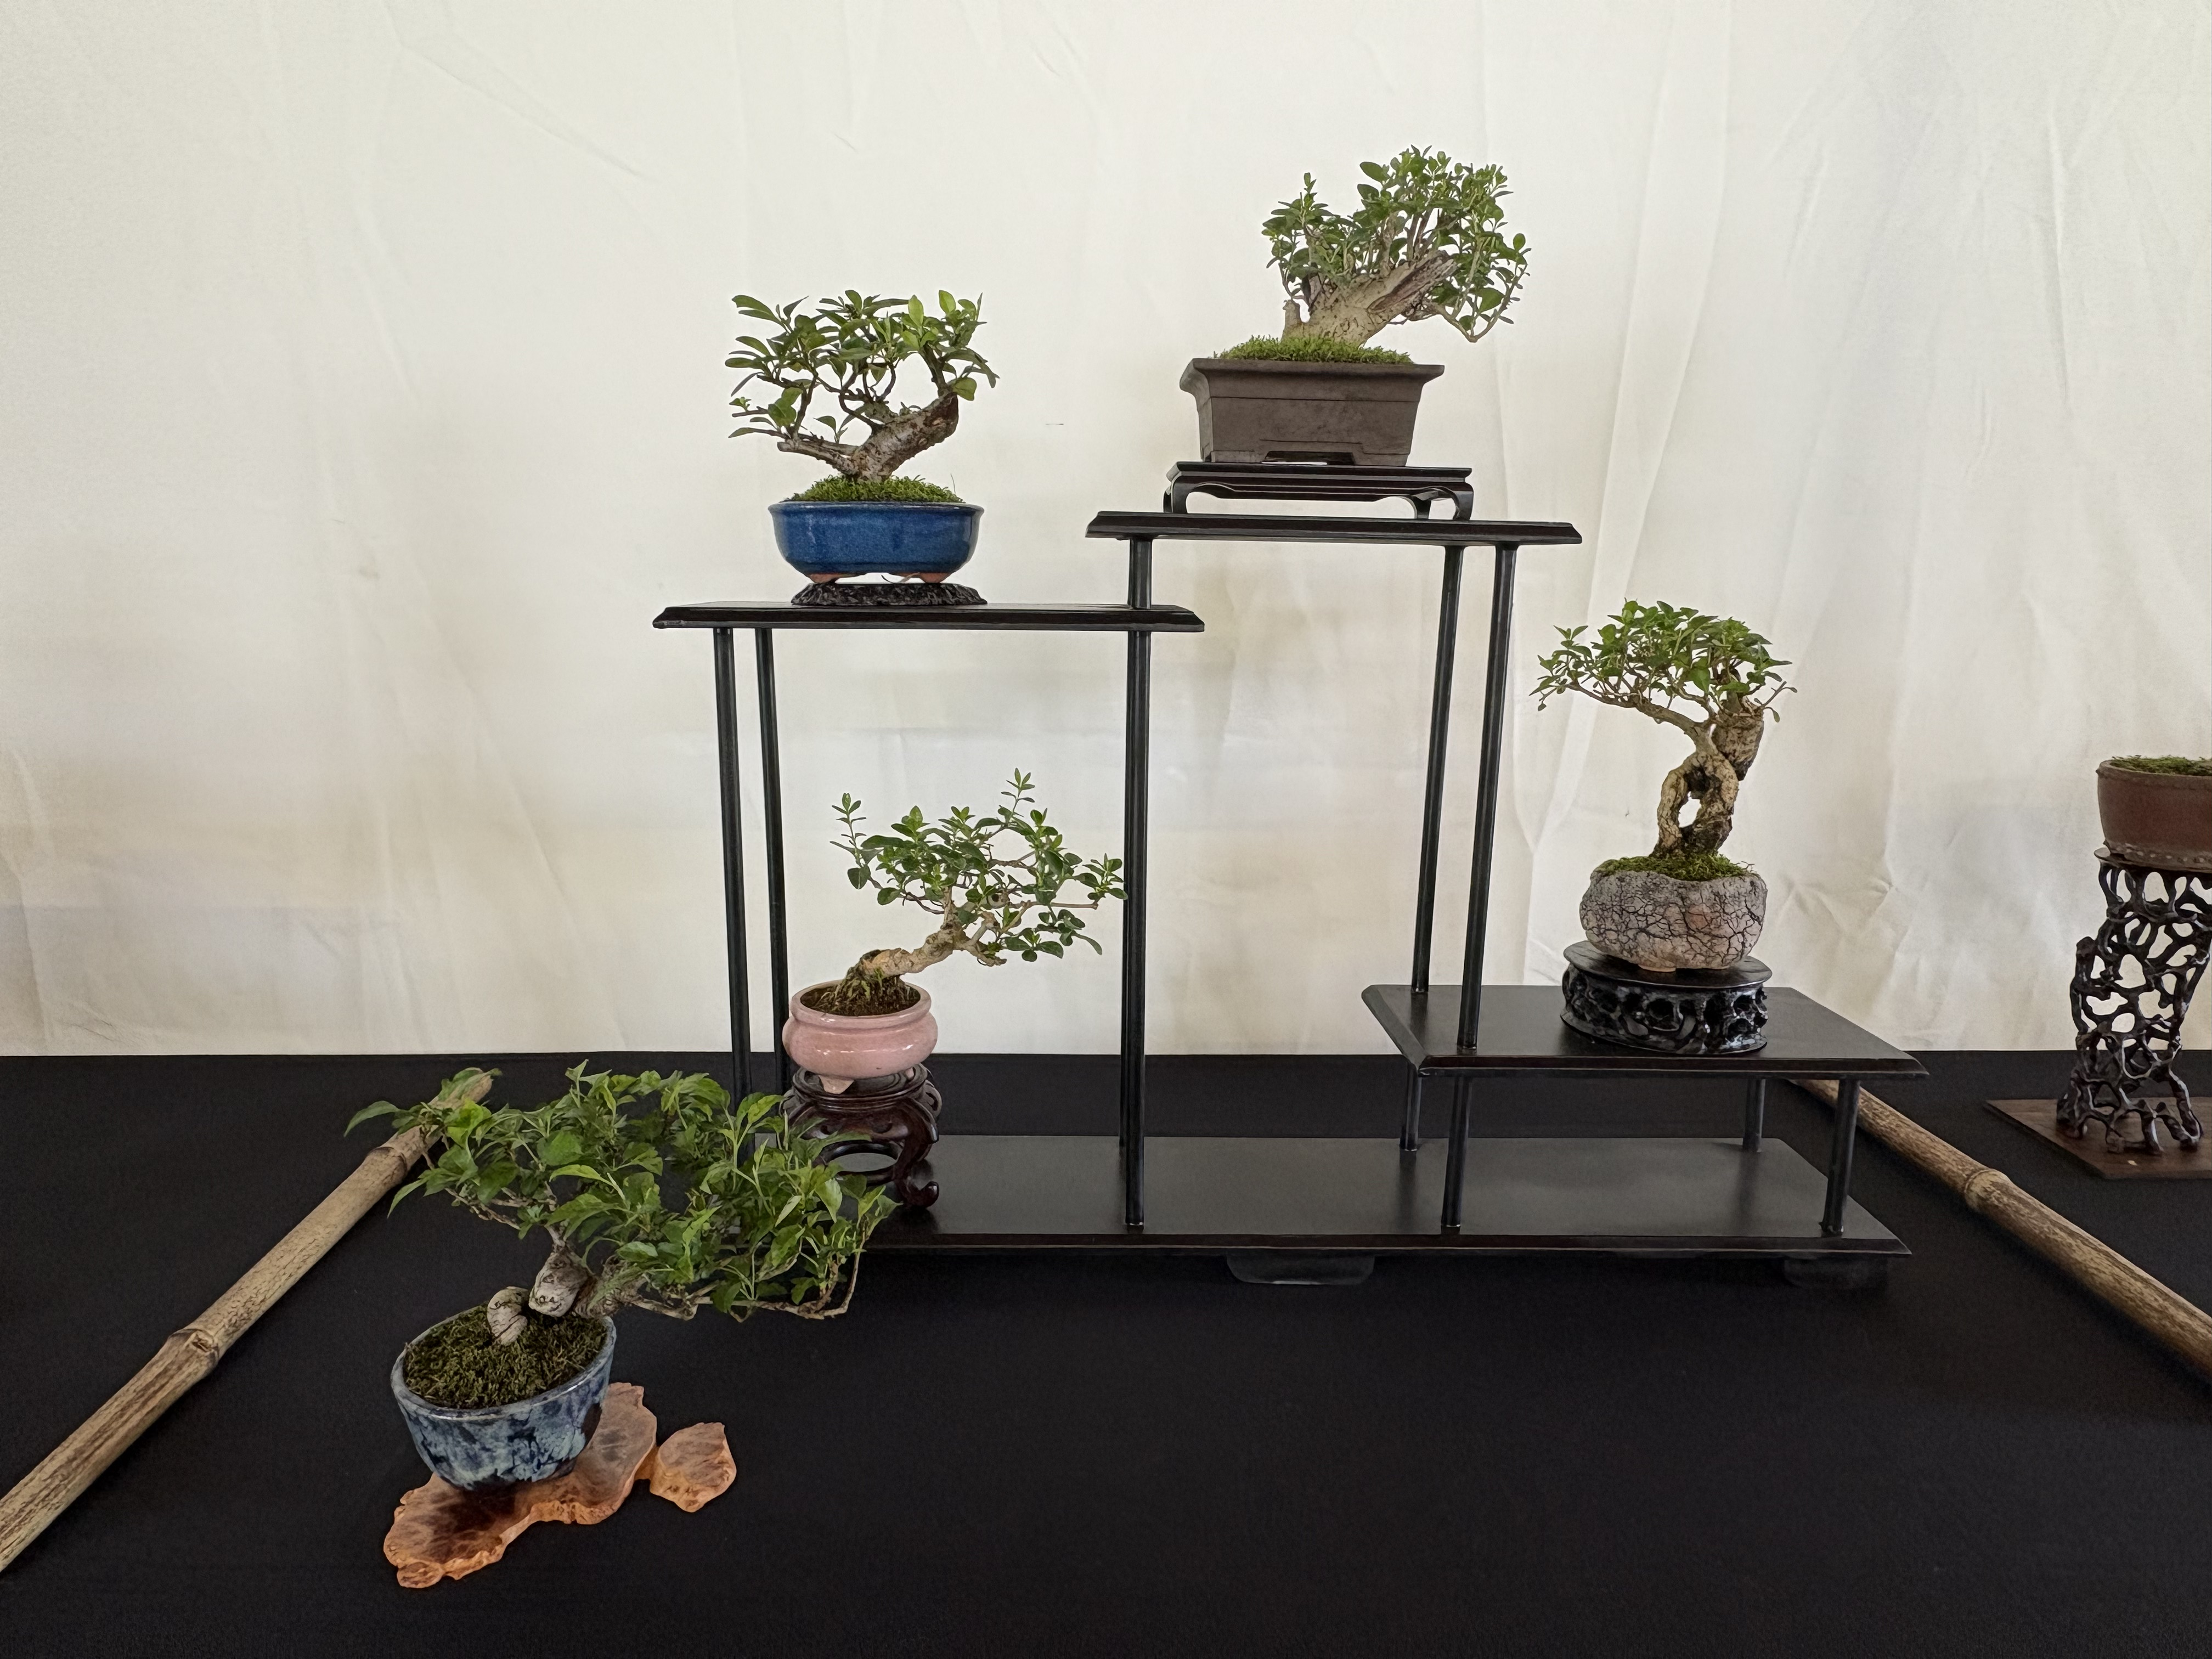
\includegraphics[width=1.0\textwidth]{2025_04/res/display_11}
% \centerline{\emph{Terry's American Sweetgum.}}
\end{minipage}\qquad
\begin{minipage}[b]{.47\textwidth}
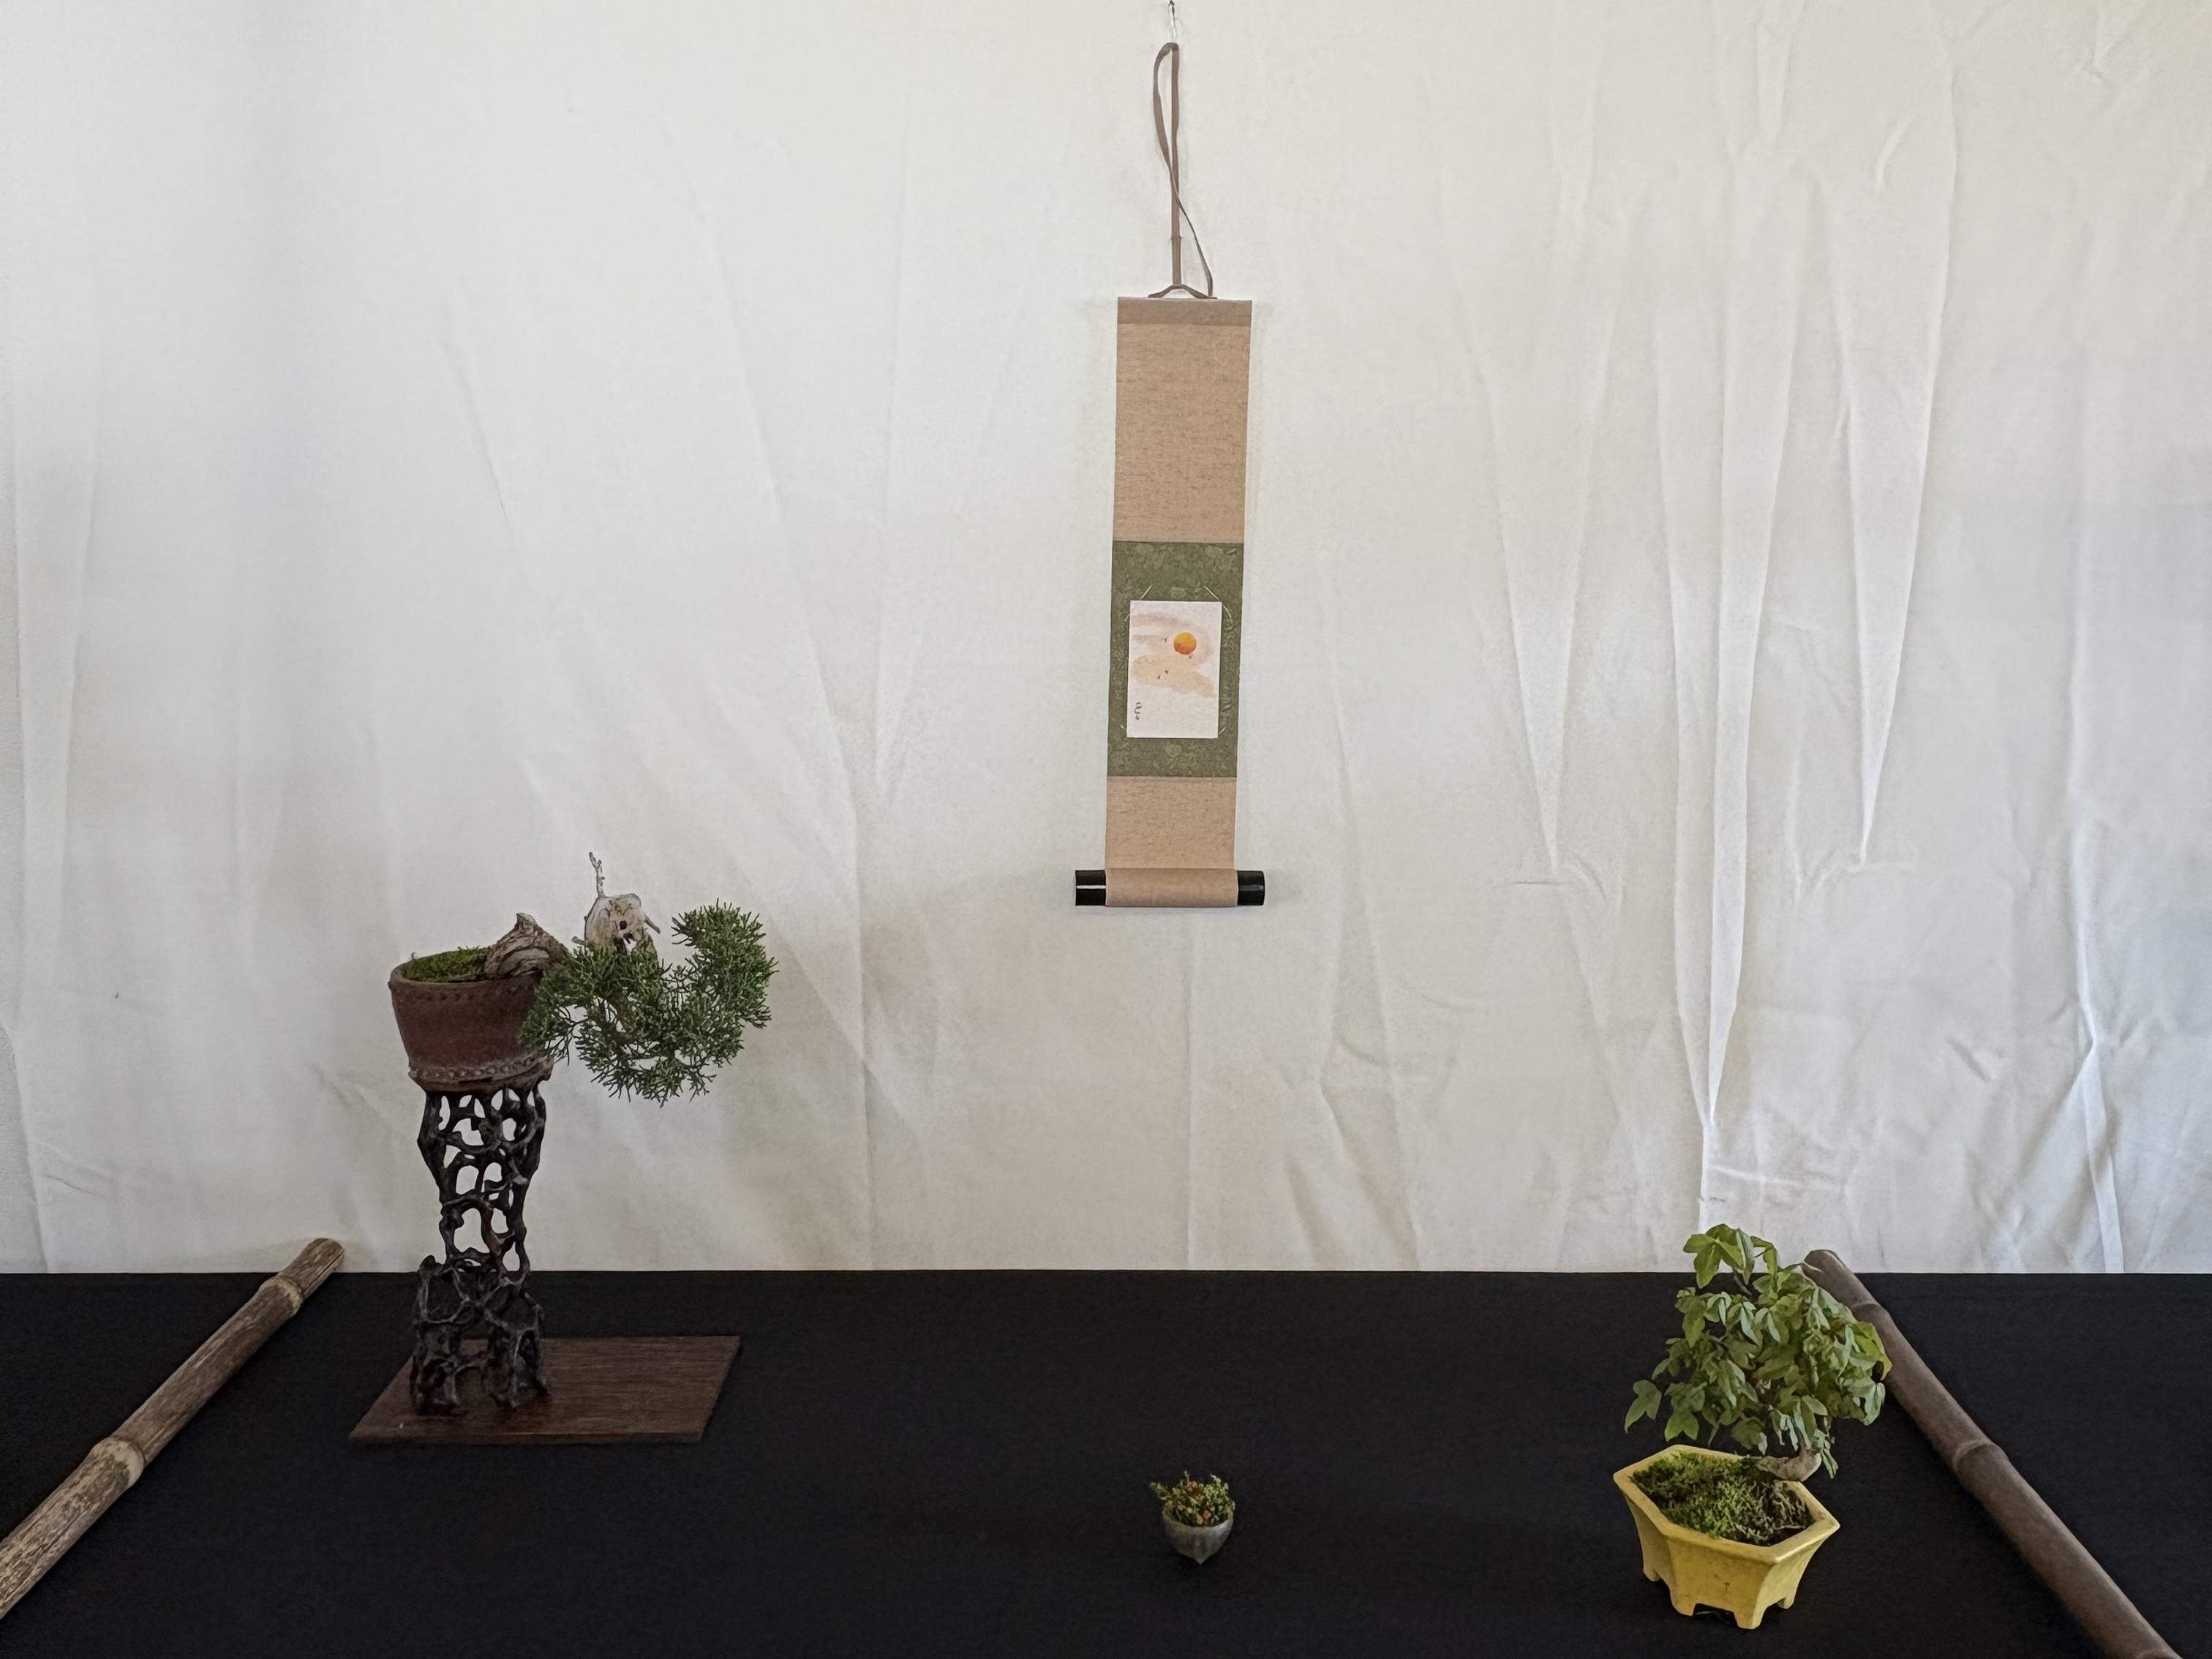
\includegraphics[width=1.0\textwidth]{2025_04/res/display_12_bis}
% \centerline{\emph{Mark's Hawthorn.}}
\end{minipage}
\medskip

% \begin{minipage}[b]{.42\textwidth}
% \includegraphics[width=1.0\textwidth]{2025_01/contest_stefano_benjamina}
% \centerline{\emph{Stefano's Ficus Benjamina.}}
% \end{minipage}

\centerline{%
\emph{The crescendo of exquisite Shohin and Mame trees, resonating through Chobham Village Hall.}%
}
\end{figure*}

\topic{\large{European and Contemporary Mame Pottery}}
\noindent
While Japan remains the centre of Mame bonsai pottery, Europe is developing its own scene.

\begin{itemize}
    \item \textbf{Peter Krebs (German potter)} --- Considered one of Europe's best, he employs a technique similar to Fujioka Yoshimura, carving pots from a single block of porcelain.
    
    \item \textbf{Thor Holier (Swedish potter)} --- Incorporates skull motifs and other macabre elements into his pots, reflecting themes of mortality.
    
    \item \textbf{Shohou Kiln (Founded in 1926)} --- Still producing bonsai pots today, maintaining a strong lineage of craftsmanship.
\end{itemize}

Alex expressed concern that younger Japanese generations are less interested in pursuing careers in bonsai pottery, as they favour modern professions over working in traditional, labour\--intensive kilns.


\begin{figure*}[!b]
\centering
\begin{minipage}[b]{.30\textwidth}
\includegraphics[width=1.0\textwidth]{2025_04/res/methods_01_bis}
\end{minipage}\qquad
\begin{minipage}[b]{.30\textwidth}
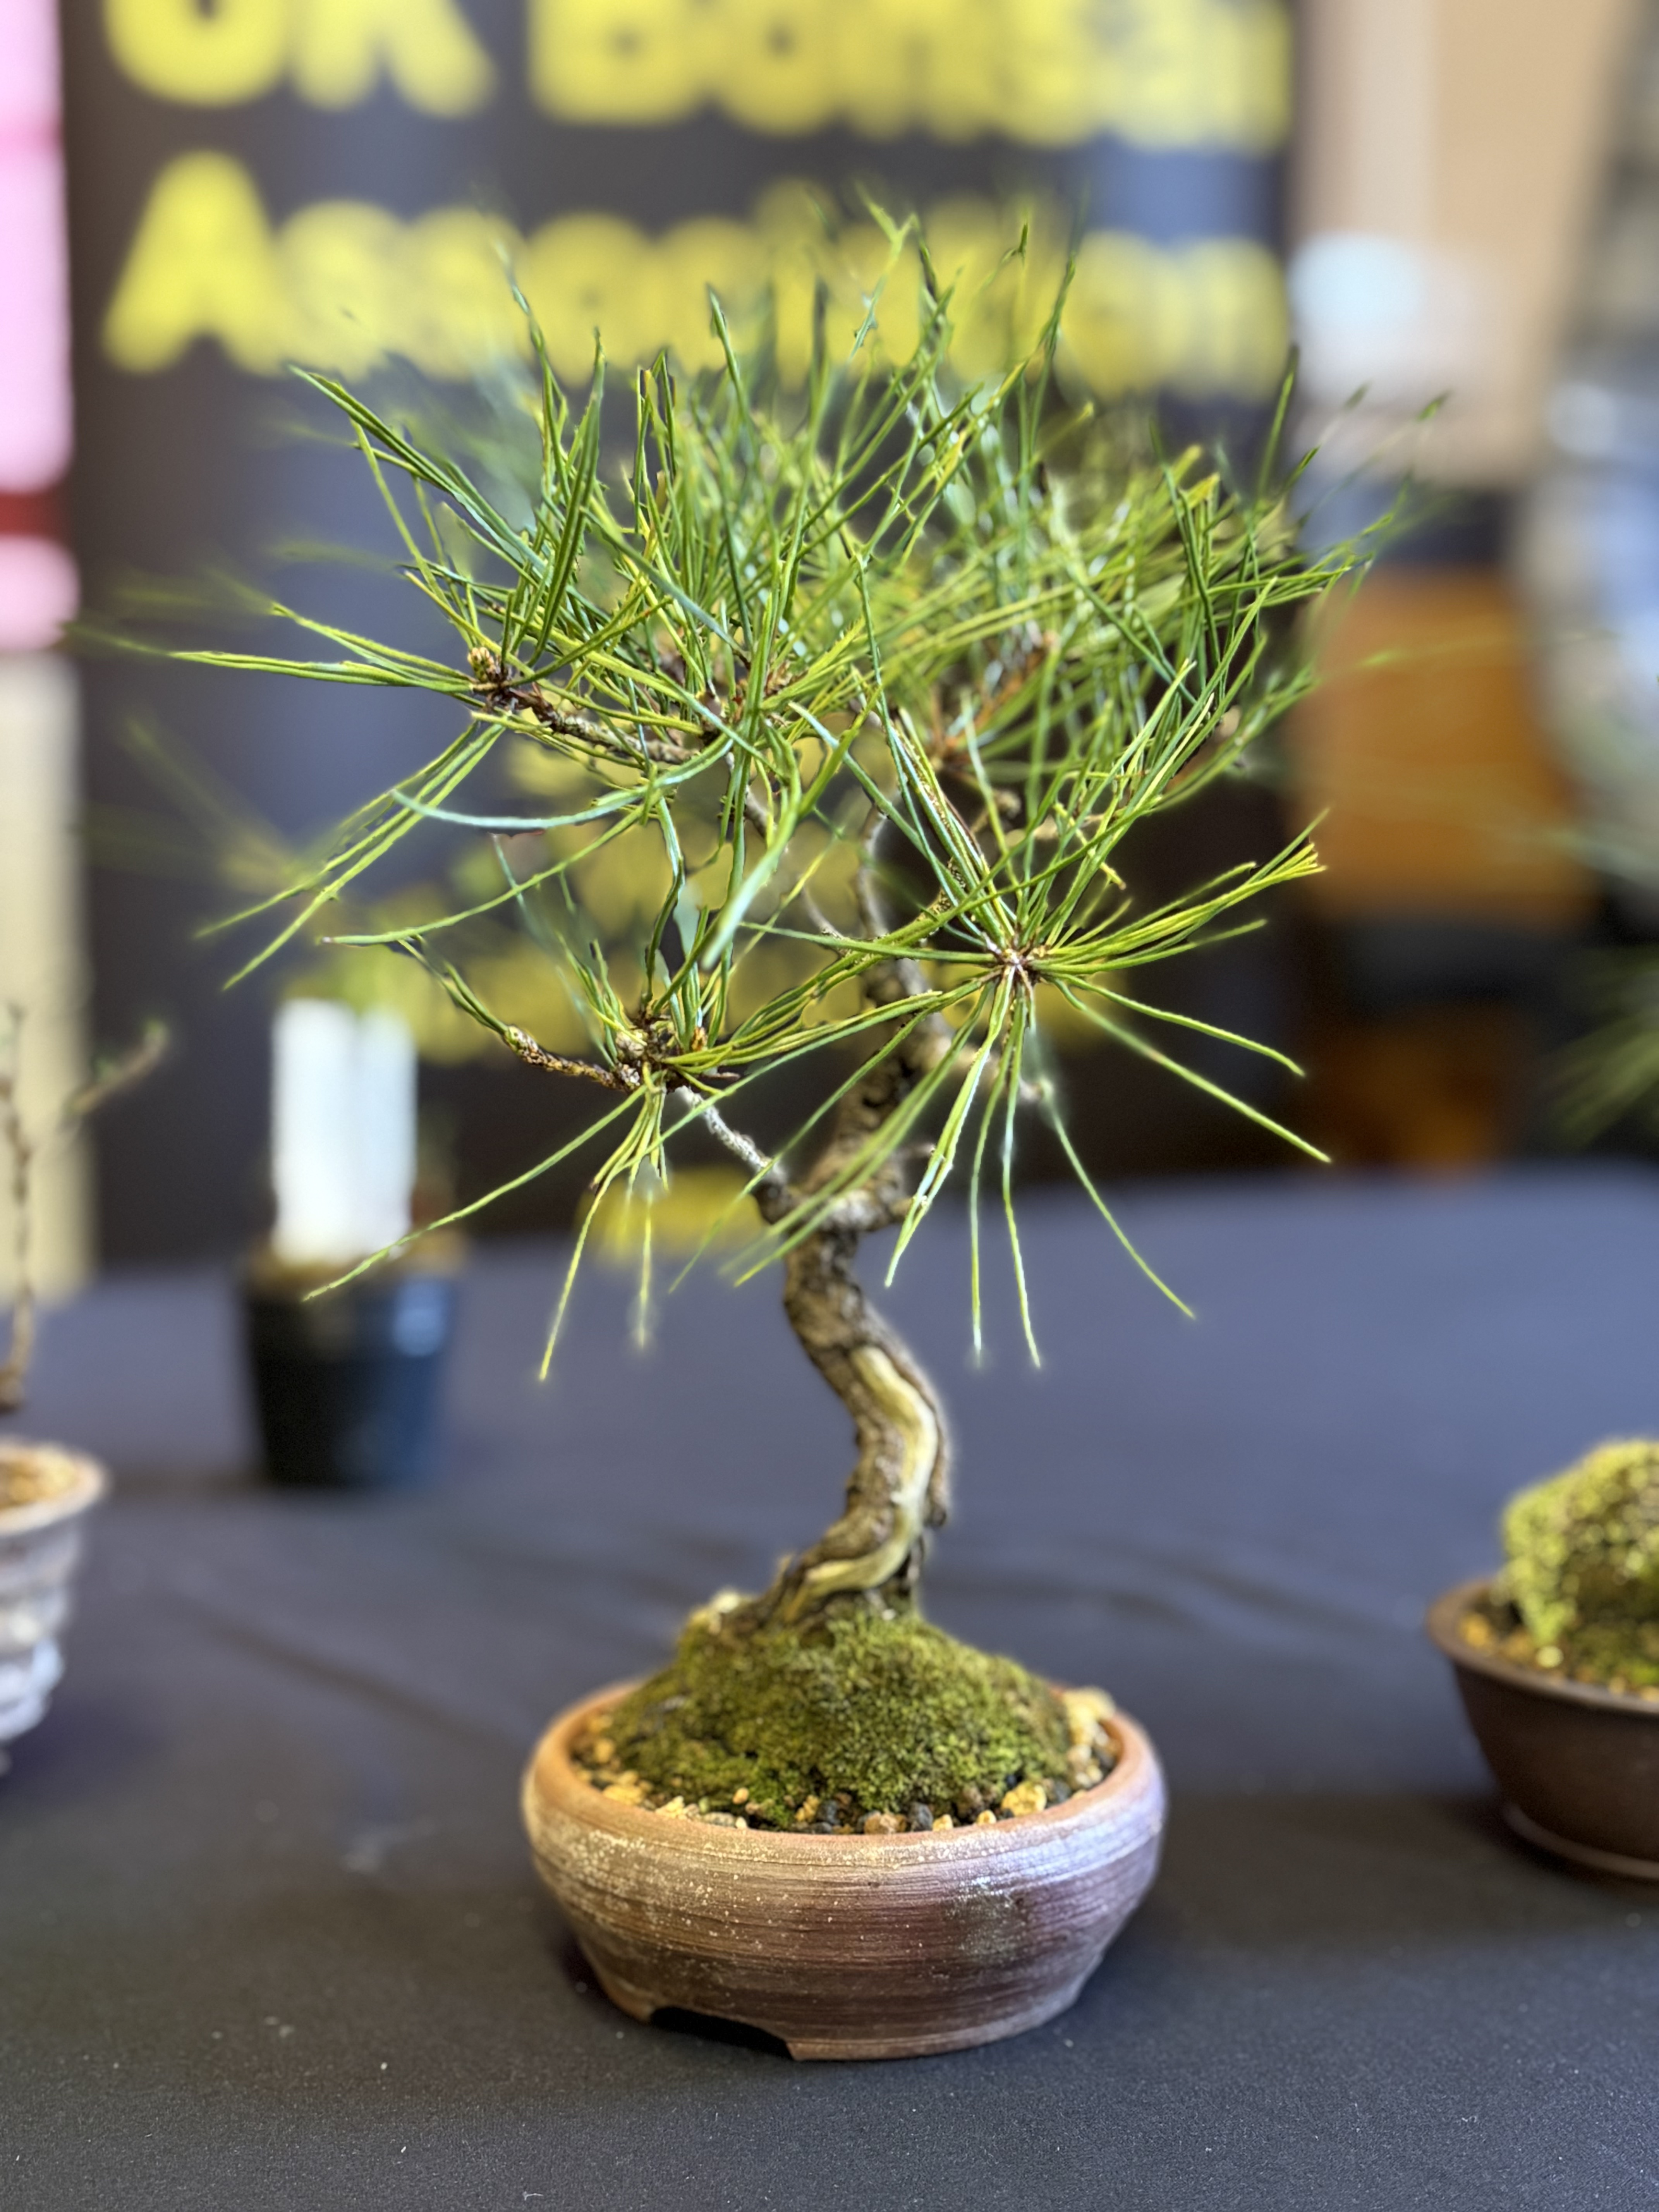
\includegraphics[width=1.0\textwidth]{2025_04/res/methods_02}
\end{minipage}\qquad
\begin{minipage}[b]{.30\textwidth}
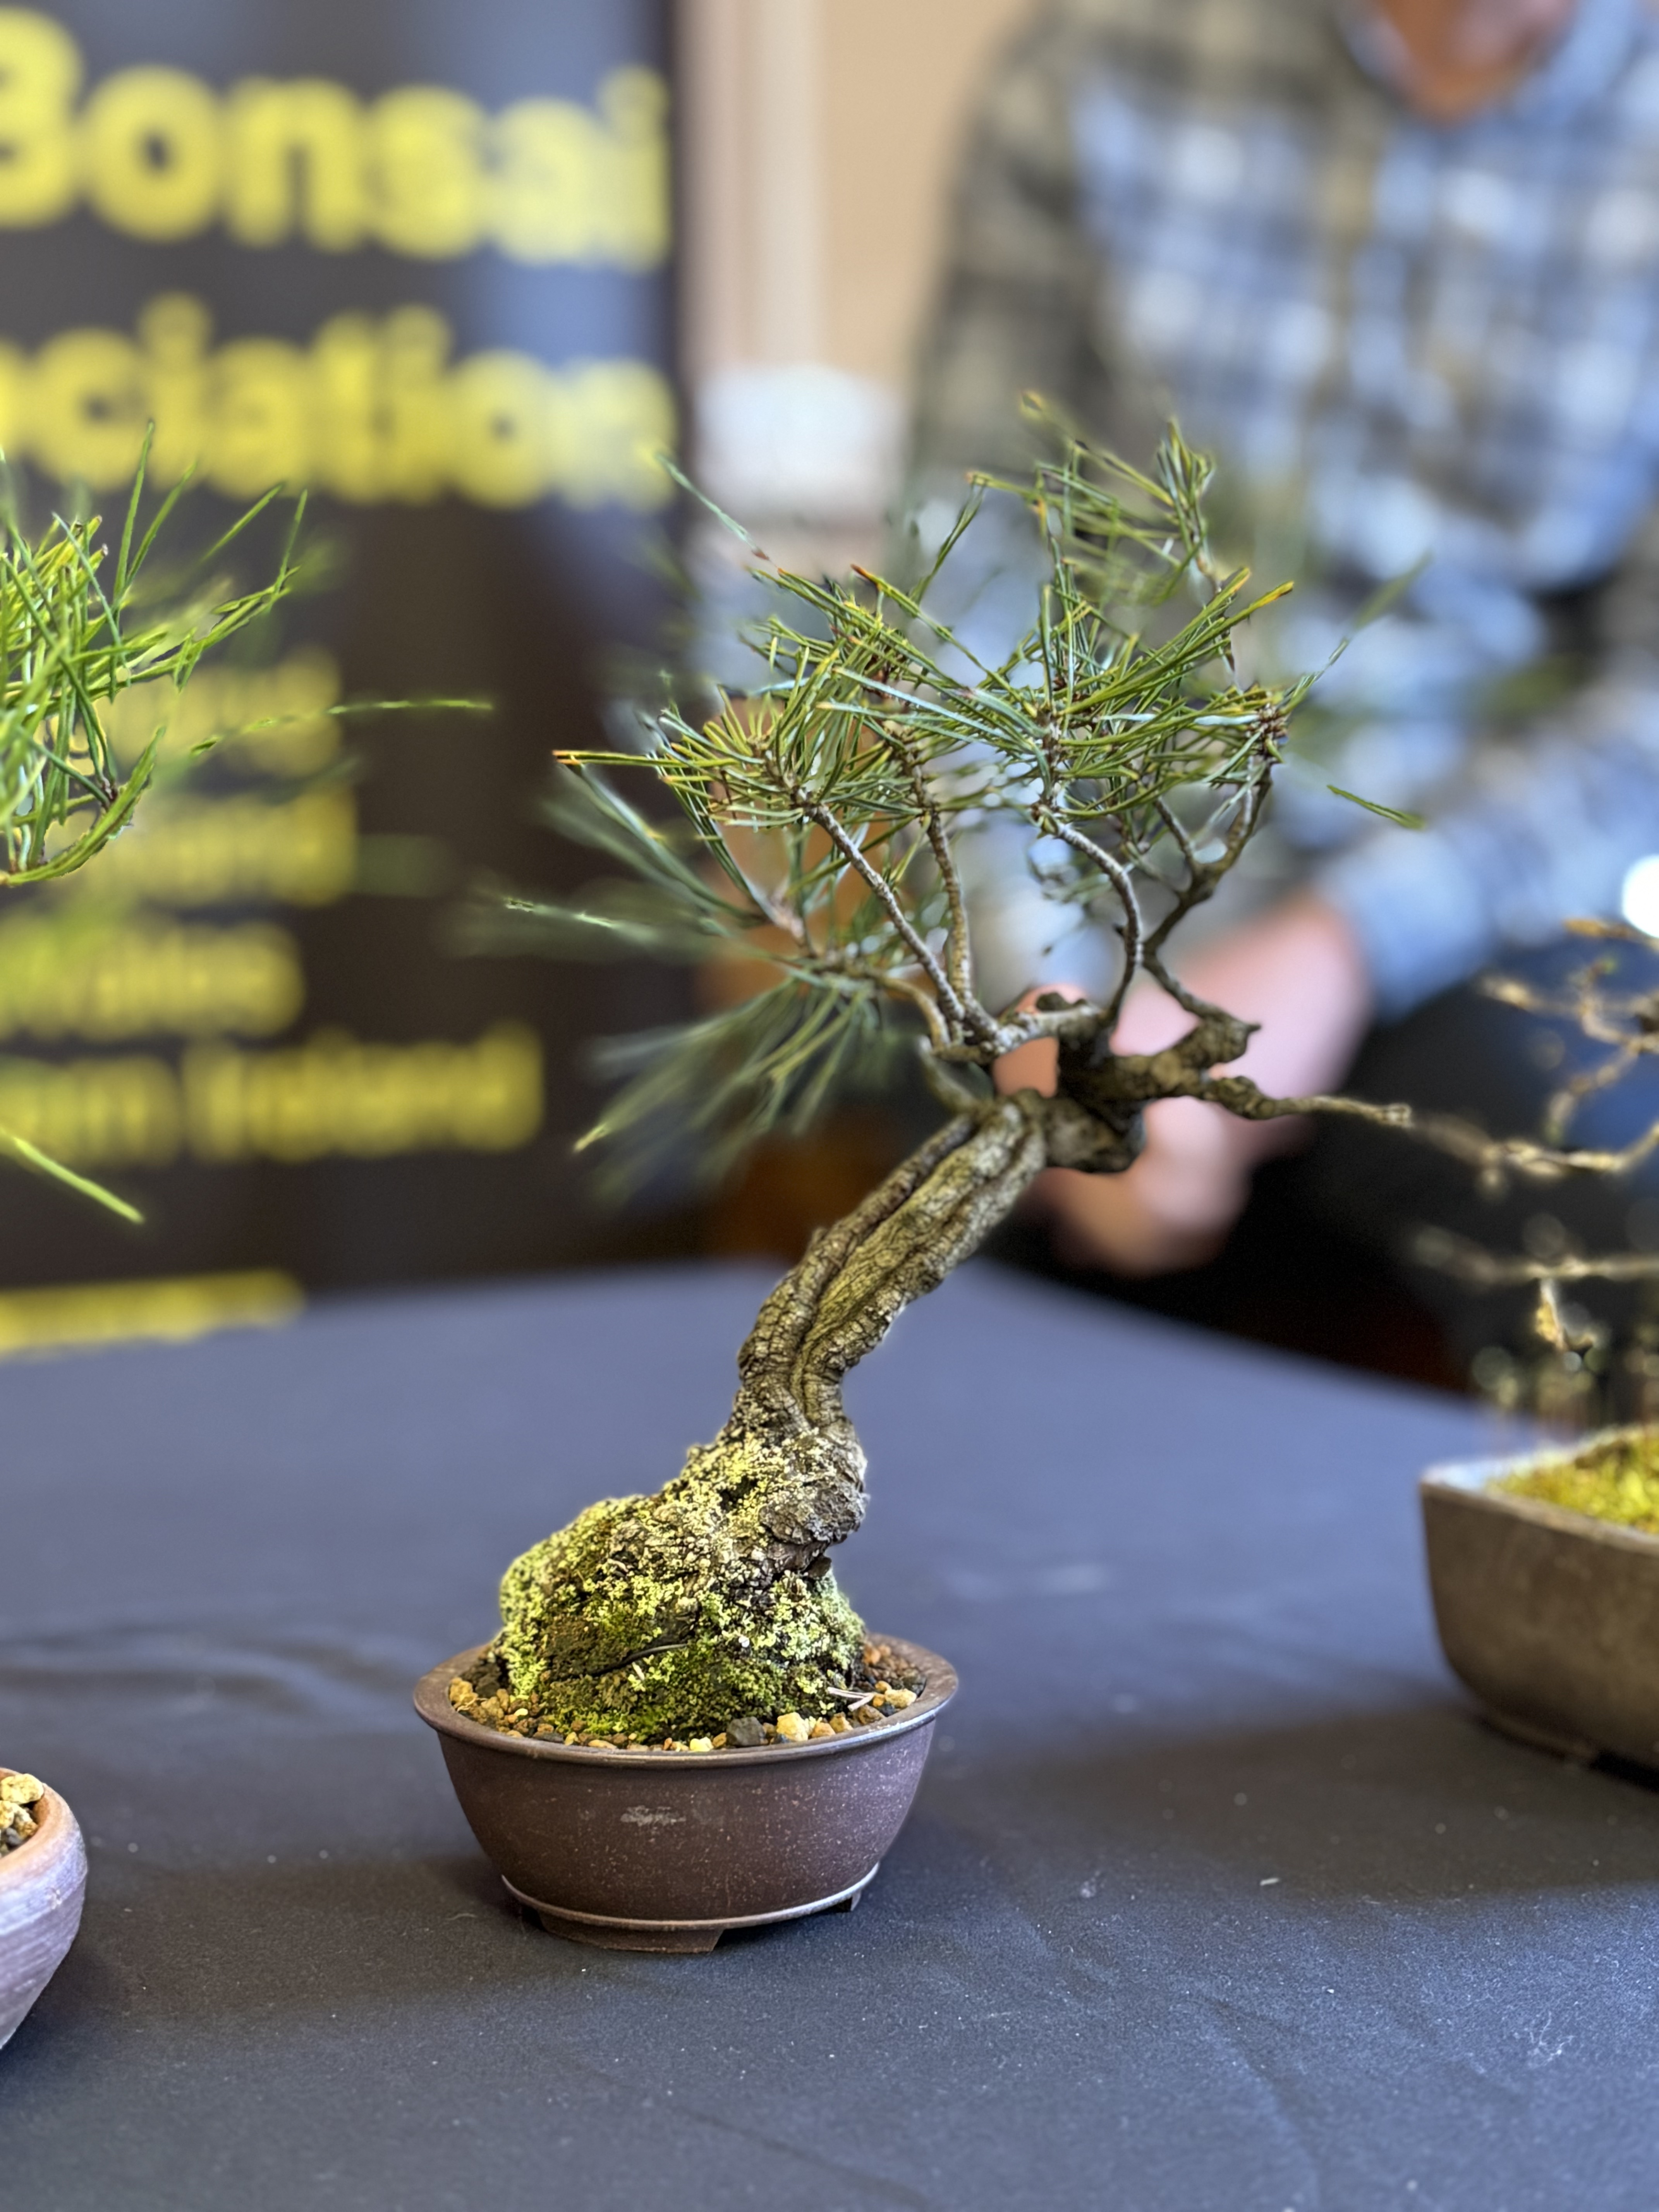
\includegraphics[width=1.0\textwidth]{2025_04/res/methods_03}
\end{minipage}
\medskip 

\begin{minipage}[b]{.30\textwidth}
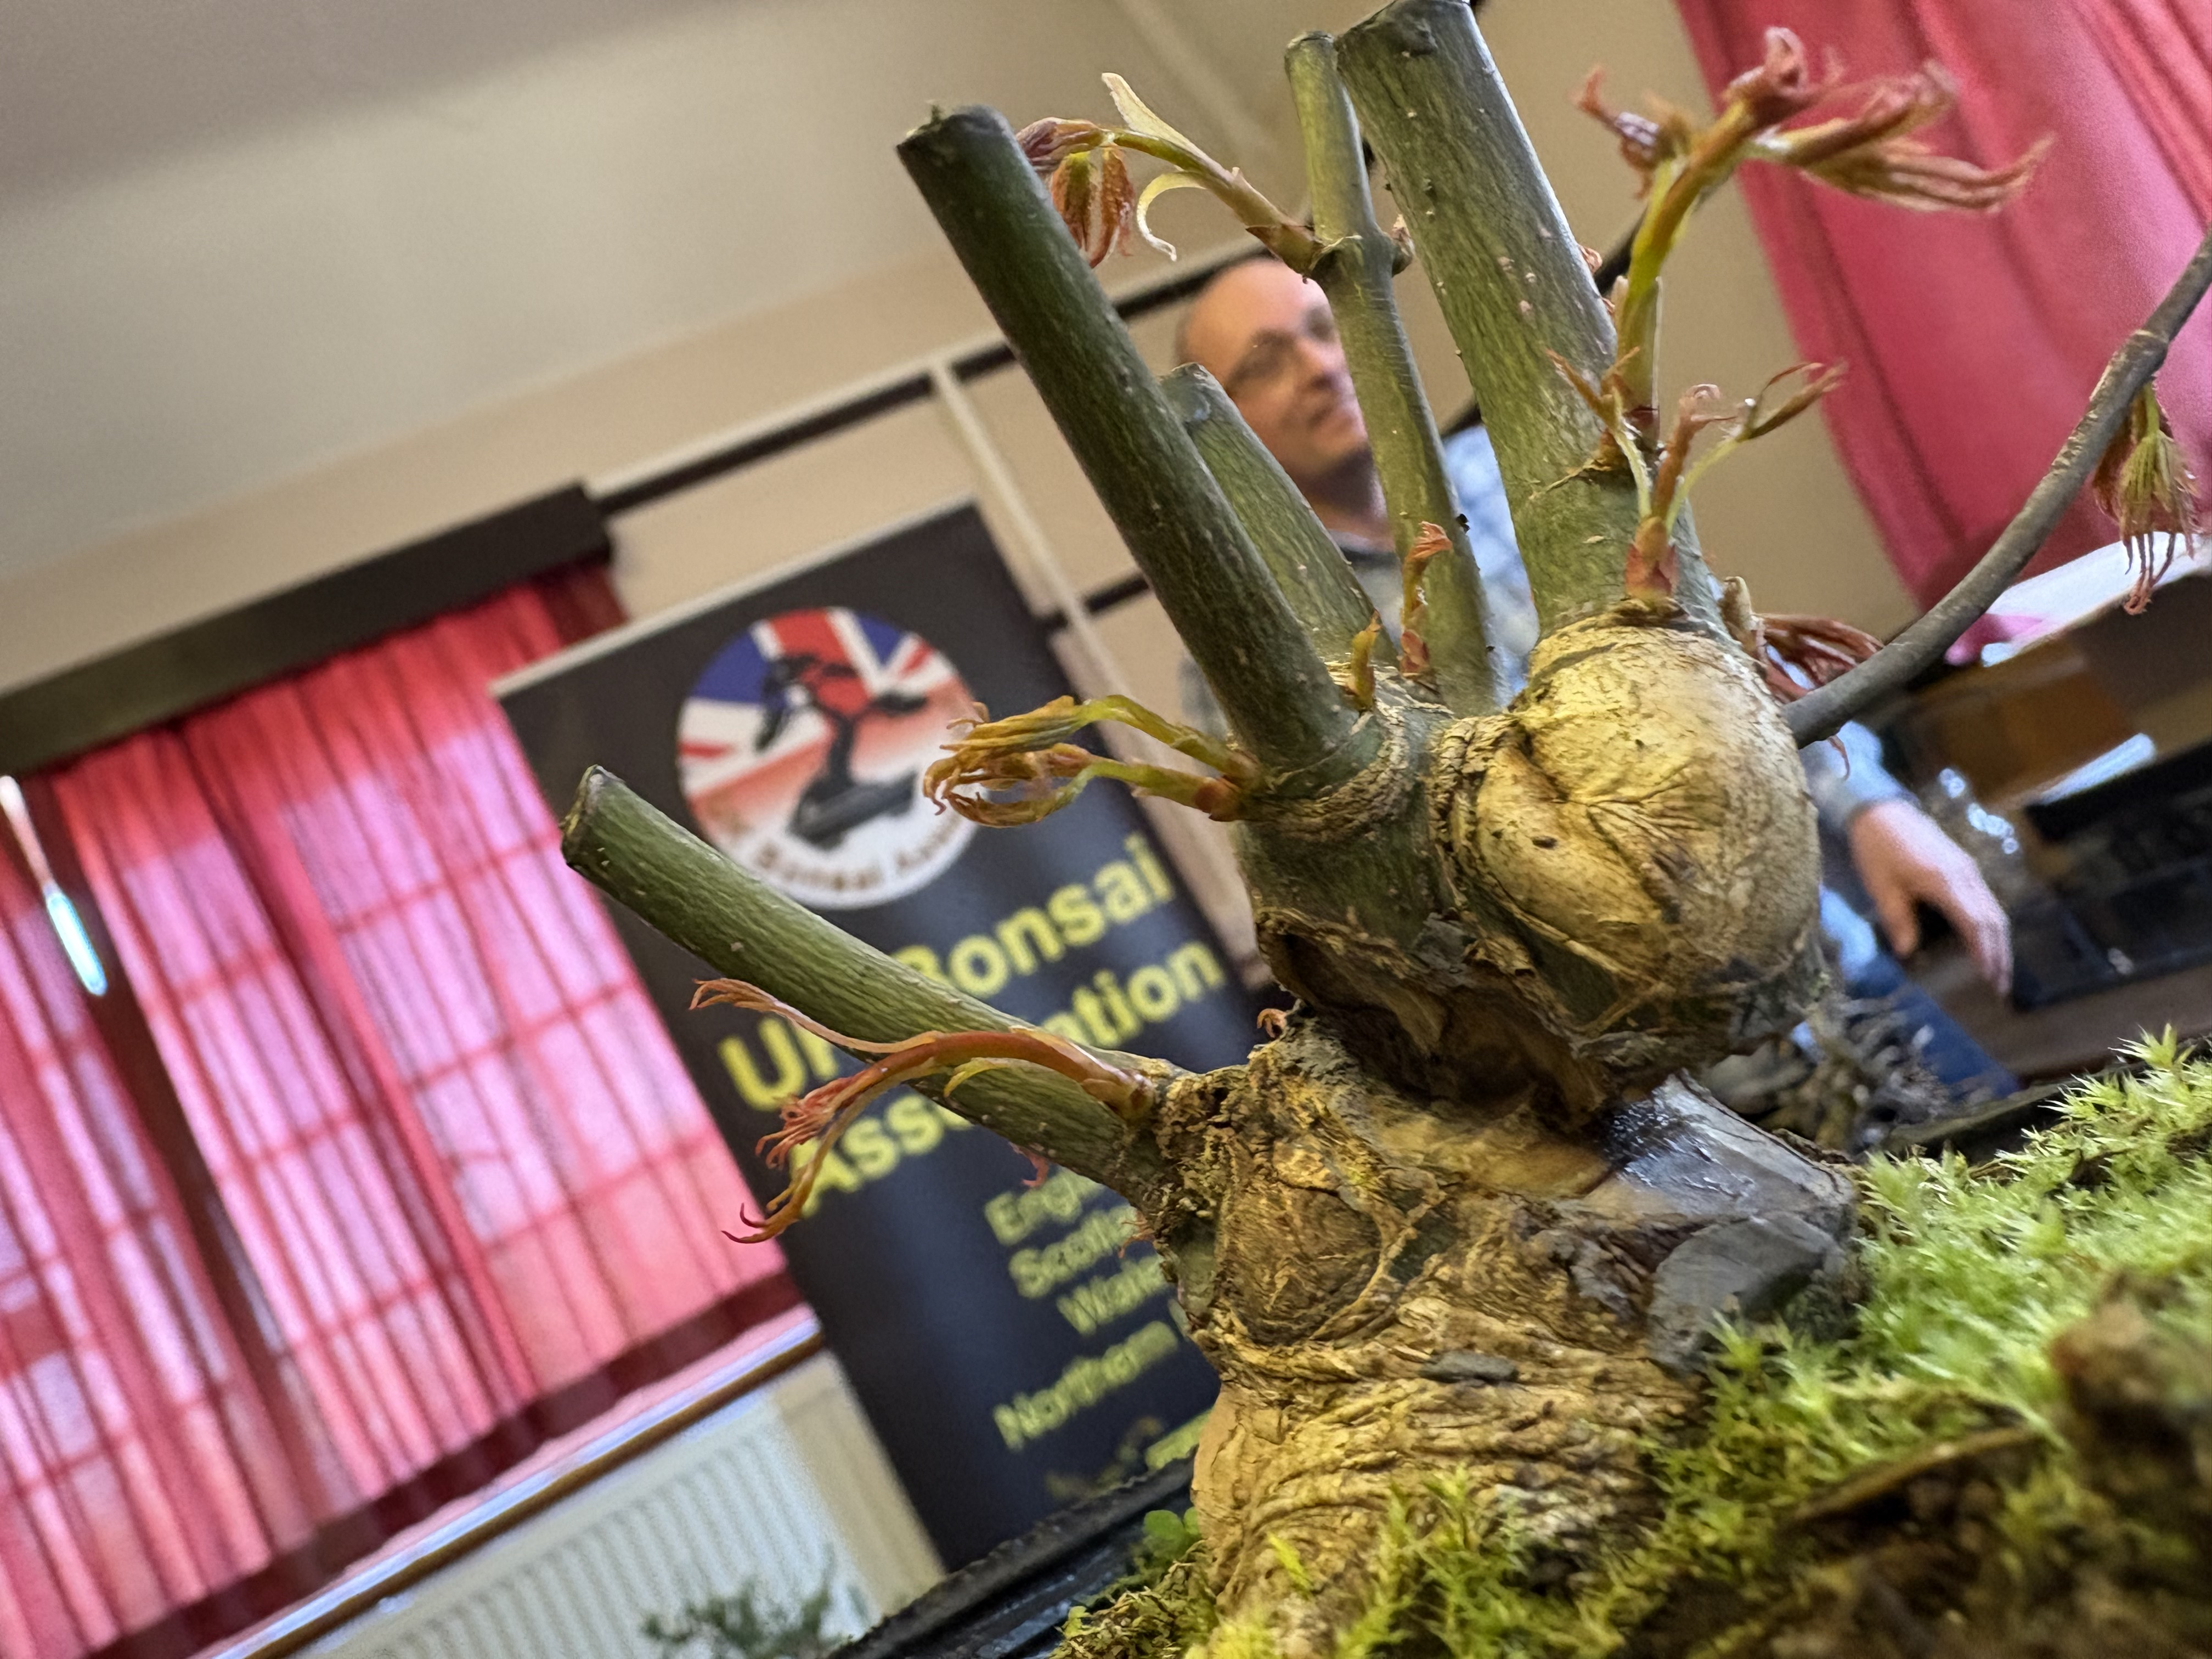
\includegraphics[width=1.0\textwidth]{2025_04/res/methods_04}
\end{minipage}\qquad
\begin{minipage}[b]{.30\textwidth}
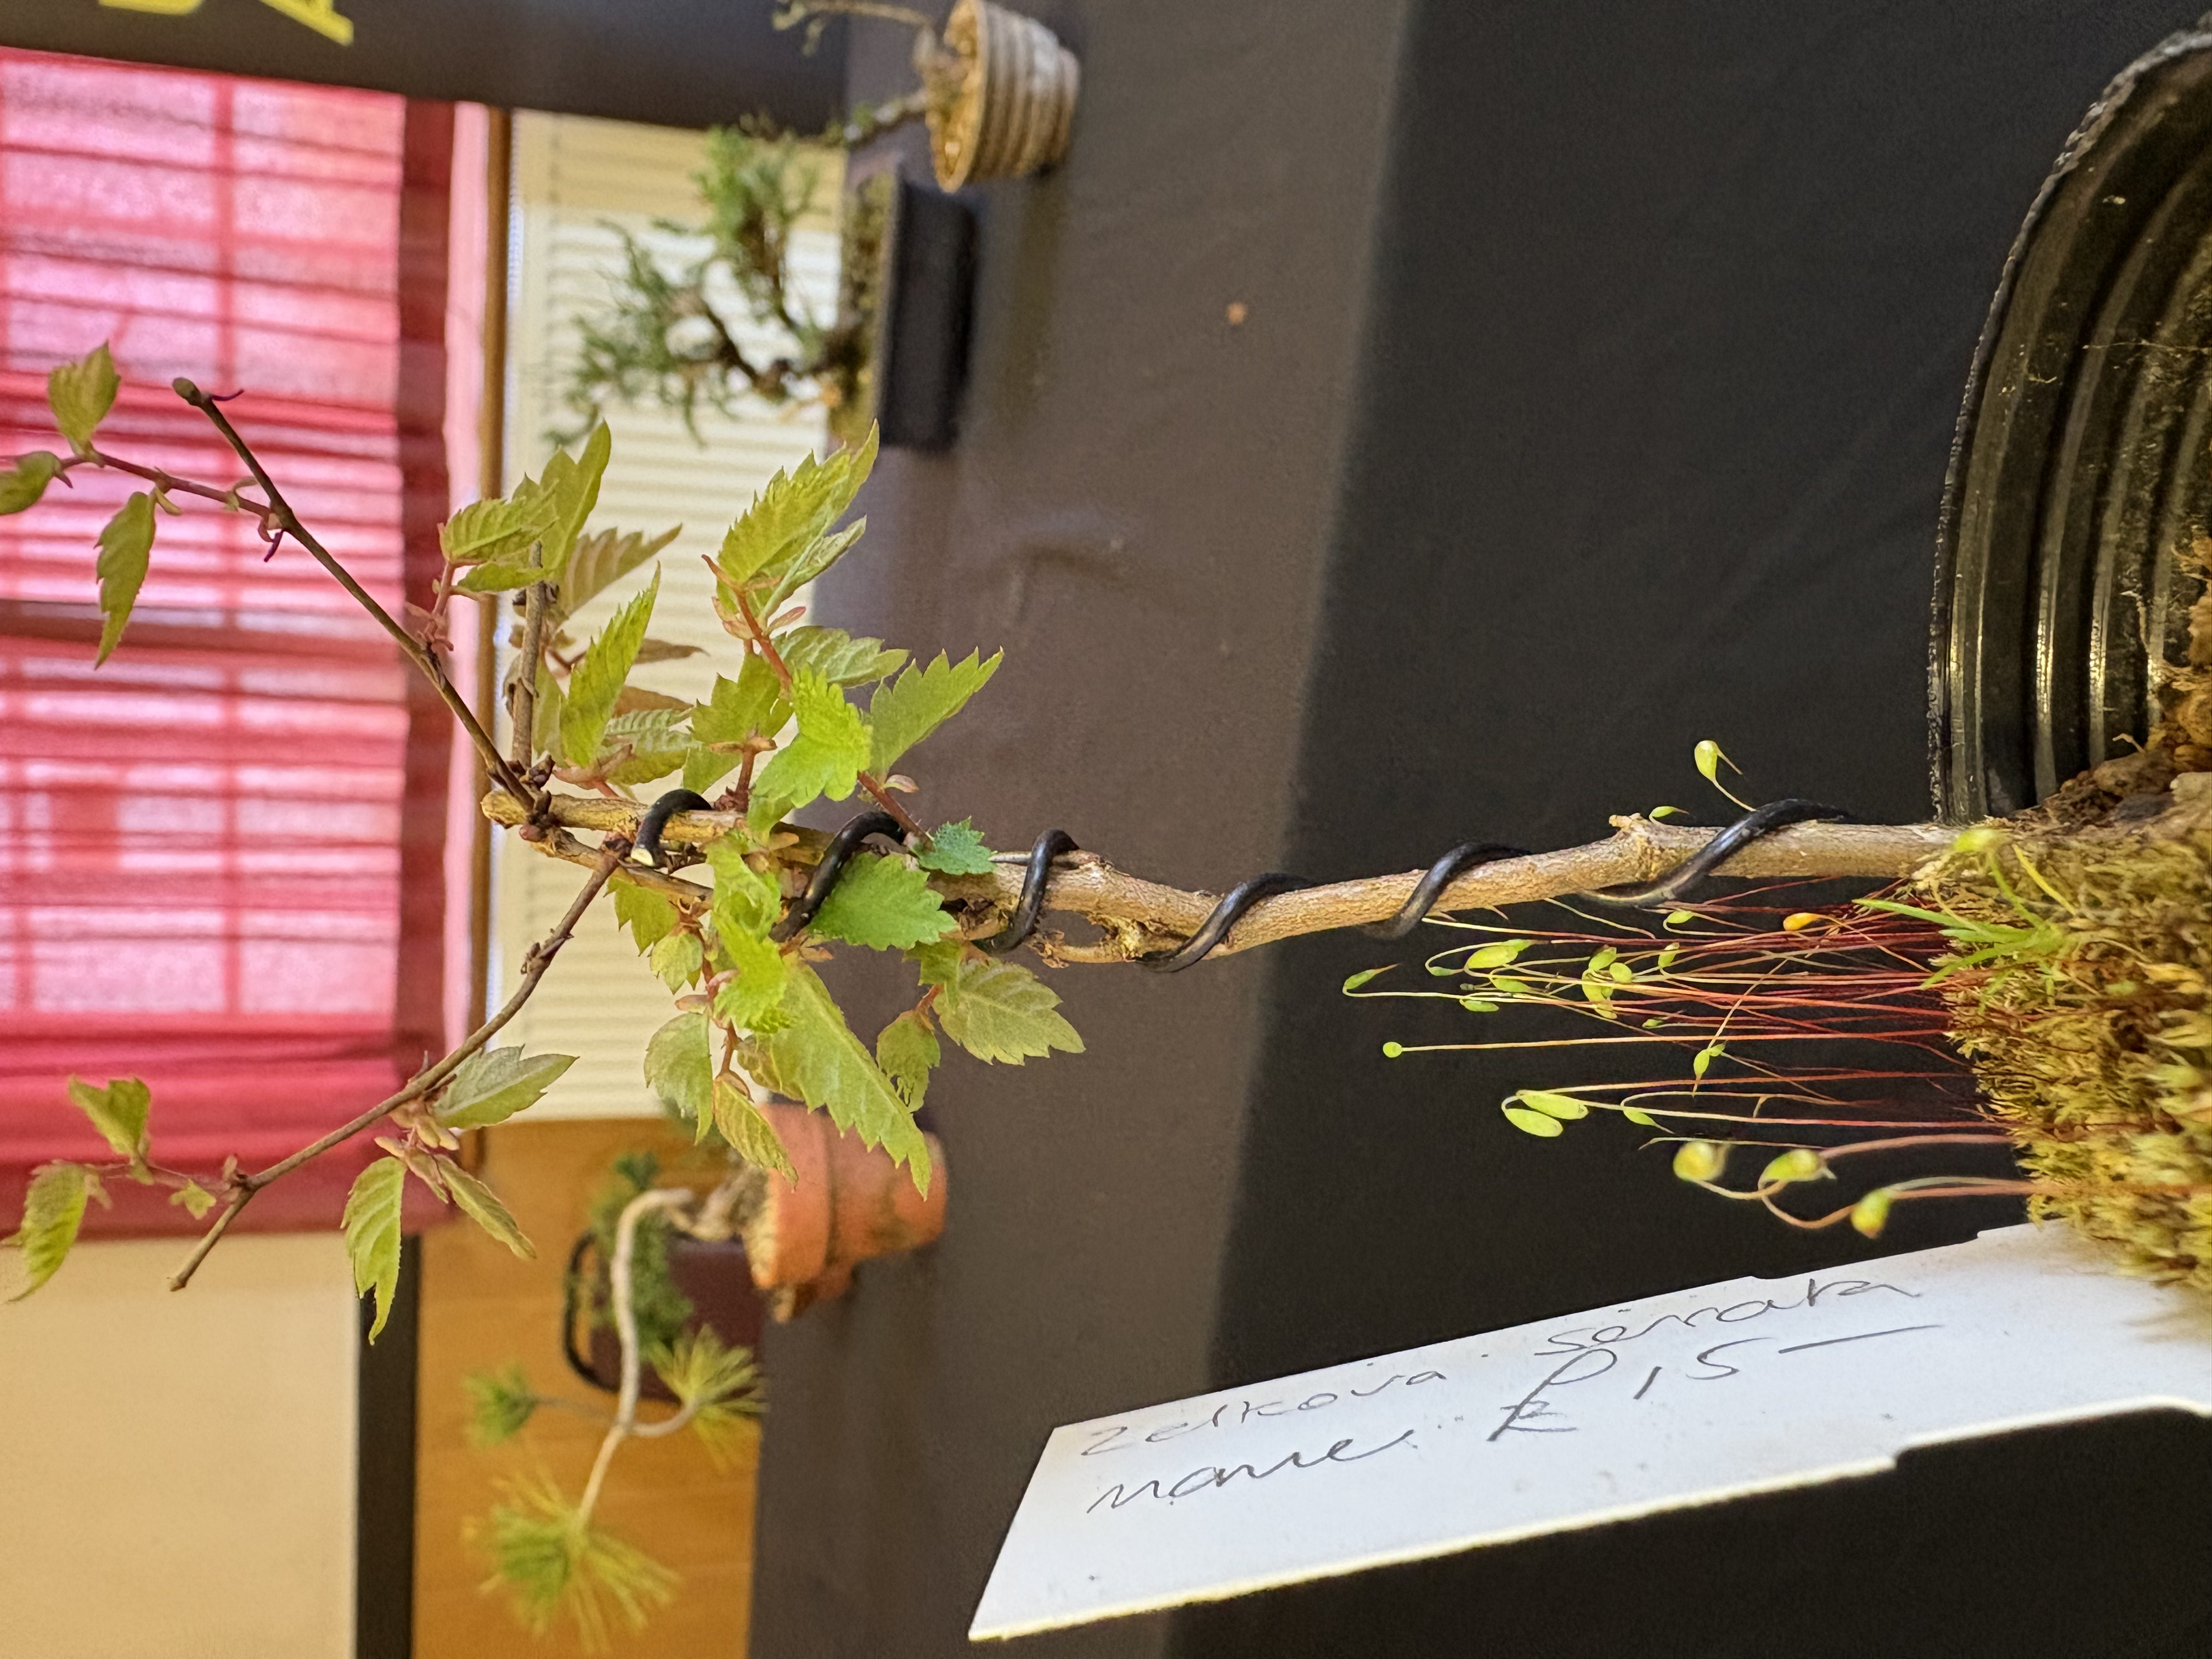
\includegraphics[angle=270,origin=c,width=1.0\textwidth]{2025_04/res/methods_05}
\end{minipage}\qquad
\begin{minipage}[b]{.30\textwidth}
\includegraphics[width=1.0\textwidth]{2025_04/res/methods_06}
\end{minipage}
\medskip 

\centerline{%
\emph{Some of the trees David Cheshire used to demonstrate techniques from his presentation.}}
\end{figure*}


\medskip

\topic{\large{The Future of Mame Bonsai Pots in Europe}}
\noindent
Alex noted that while tree prices are rising, pot prices have seen some fluctuations. 

When asked about his own collection, Alex revealed that he owns \textbf{around 3,000 pots} and \textbf{about 150 trees}, spread across two gardens.
Despite the increasing market value of his pots, he has no intention of selling them, as he sees them as irreplaceable works of art.

\closearticle
\columnbreak
